% Architecural design section, to be included in architecture.tex

\section{Architectural design}
\label{sect:arch}

\subsection{Overview}

\subsubsection{High level architecture}
Figure \ref{hwarch} shows what machines are going to be used for the system: most components are replicated to both increase performance (through the use of load balancers) and reliability, as one machine can take over the work of the other in case of fault. The logical layers are:
\begin{itemize}[itemsep=-1mm, topsep=-1mm]
	\item Presentation: realized by the clients, either the application or the web browser
	\item Logic: covered by the web servers and the application servers
	\item Data: consists in the database servers and their DBs
\end{itemize}
\vspace{.5\baselineskip}
The tiers of the system are illustrated more precisely in Section \ref{sect:deploy}.

\begin{figure}[h]	
	\centering
	\includegraphics[width=\linewidth] {deployment_diagrams/hw_arch}
	\caption{High level architecture of the system}
	\label{hwarch} 
\end{figure}

\subsubsection{Class diagram}
A class diagram of the model of the application is visible in Figure \ref{class}; it is more detailed and presents only classes that will be developed with respect to the higher-level one shown in the RASD; it corresponds to the core system residing on the application server.
Getter and setter methods have been omitted for space reasons, but they are present for every attribute except user passwords.

Classes relative to users represent the way they interact with the application; the e-Customer can therefore take all the actions described in the previous document, while the Store Manager (also through the Store class) can control every aspect of entrances and of their activity.

\subsubsection{ER diagram}
Figure \ref{er} shows the ER model for the application's database. The tables are mapped to some classes in the class diagram (that adds some generalizations).

\begin{landscape}
	\begin{figure}[p]
		\centering	
		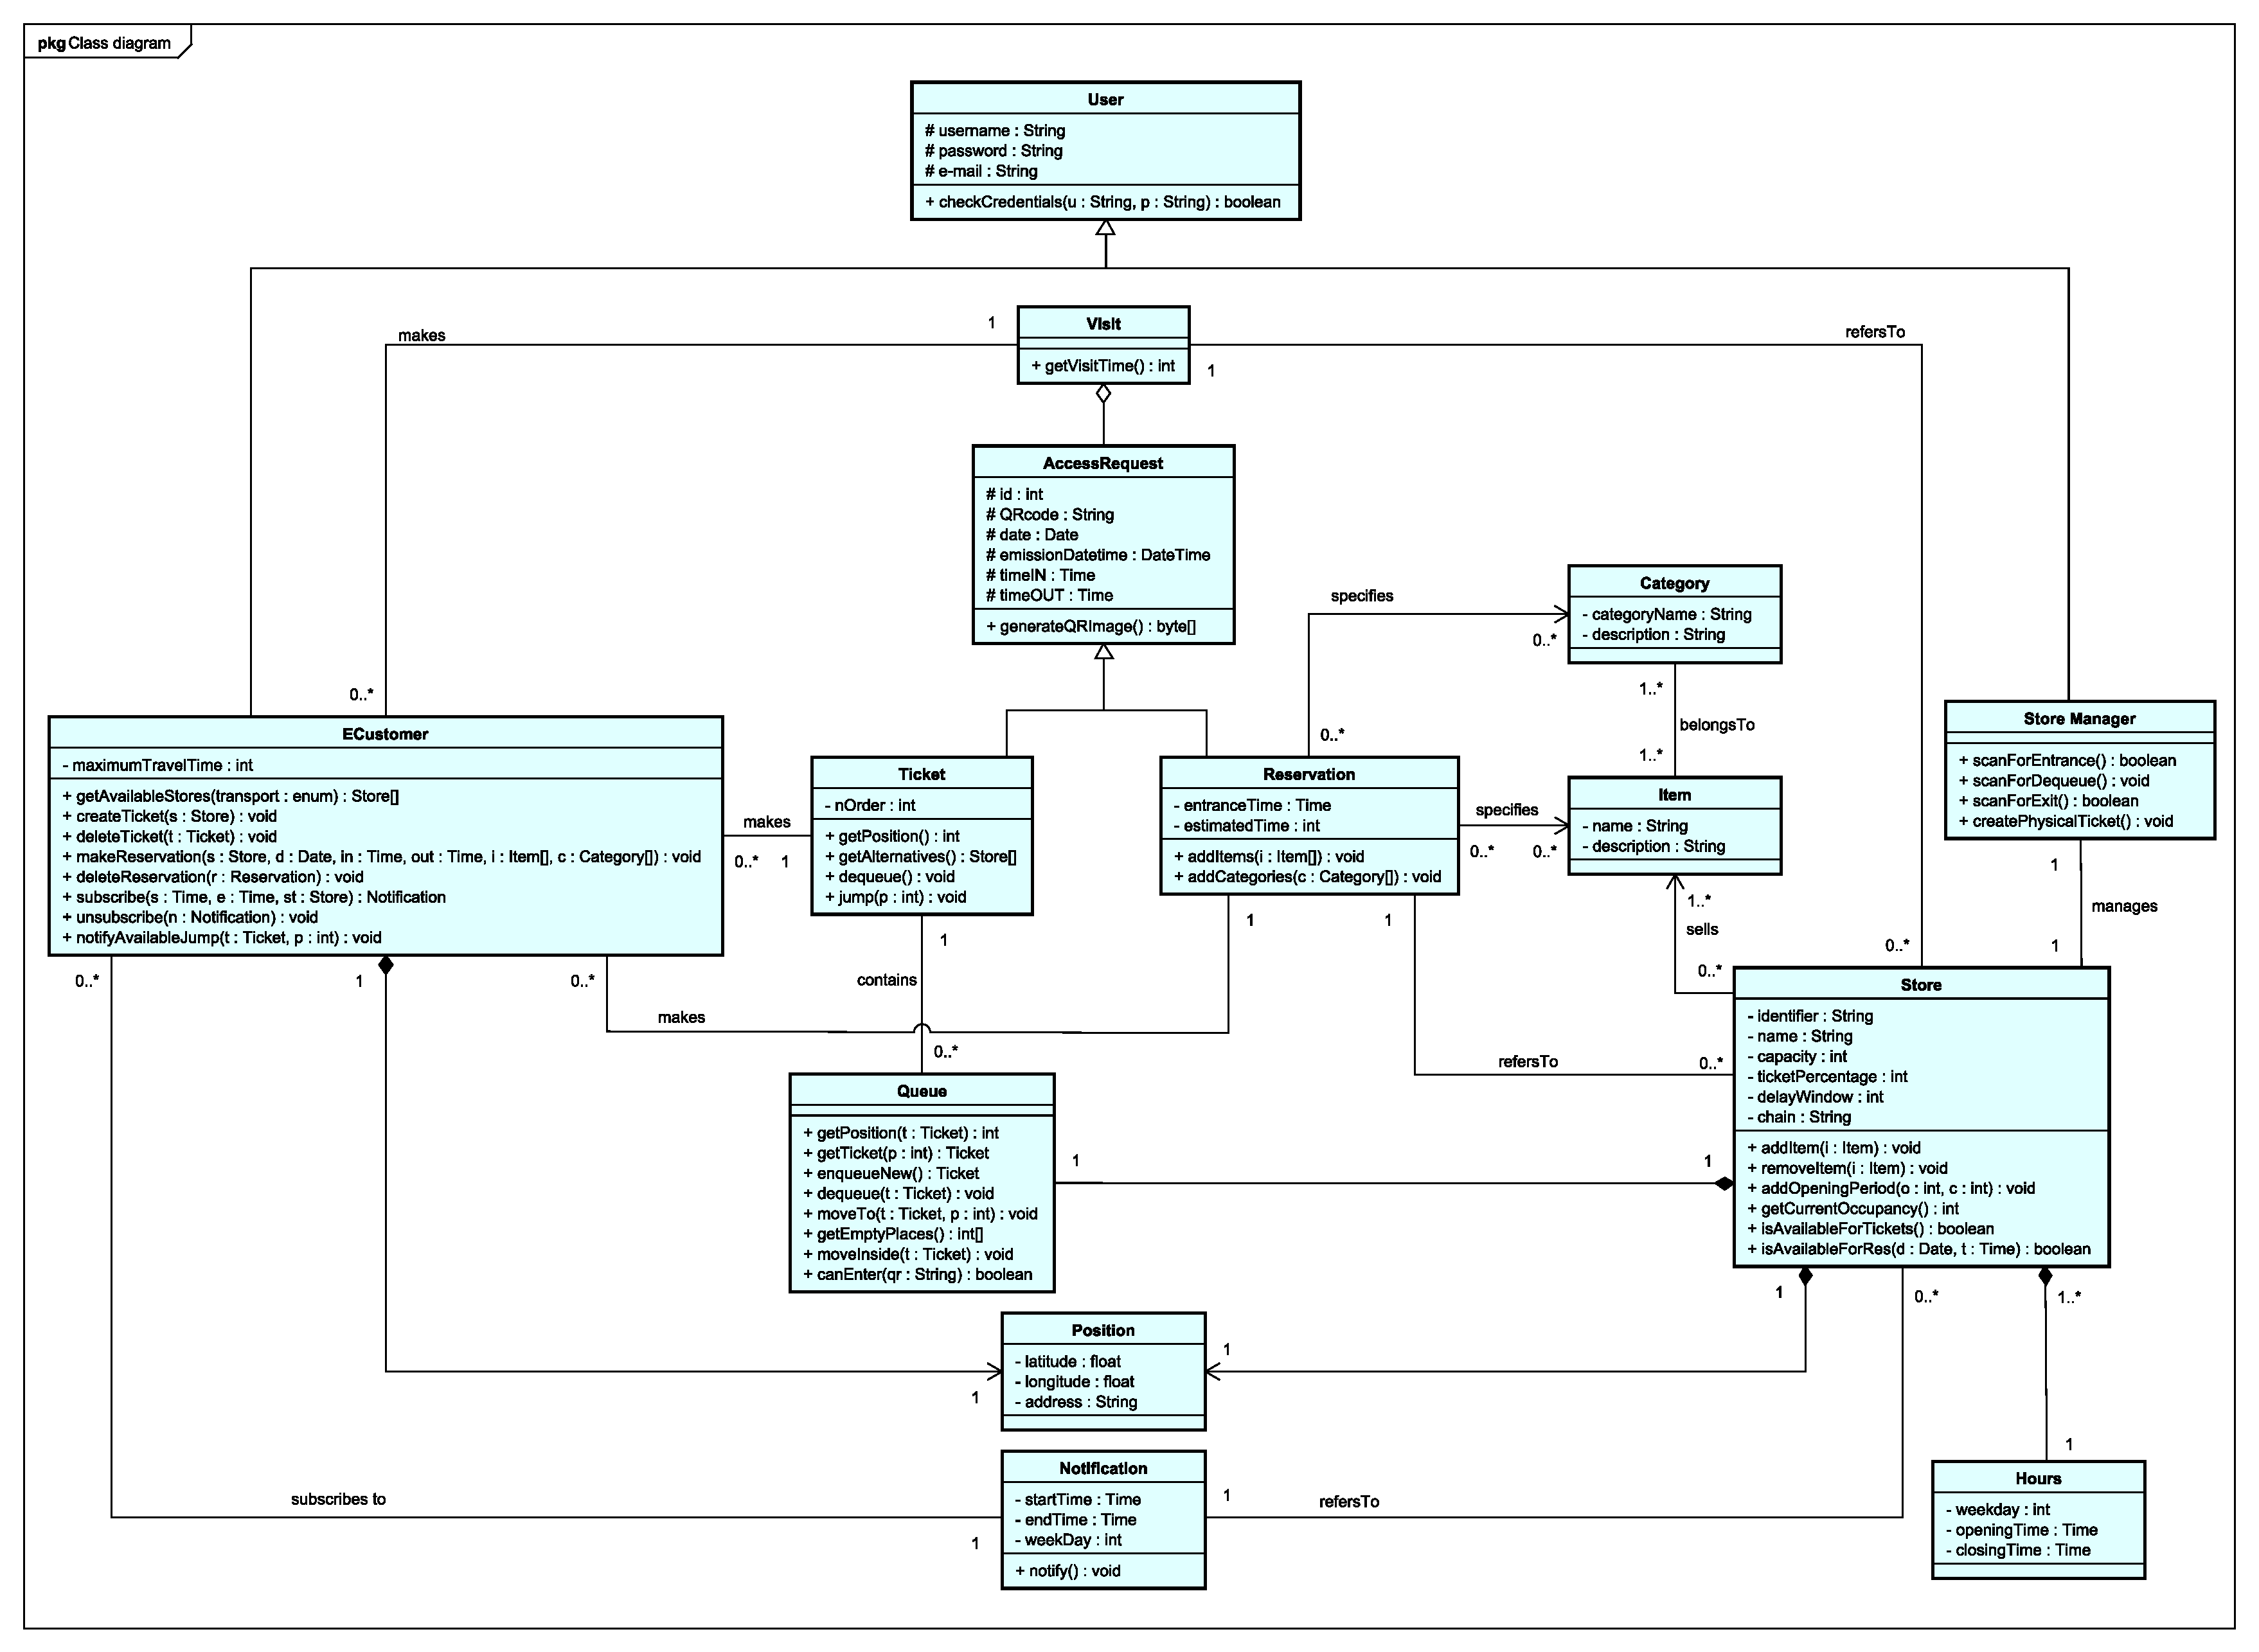
\includegraphics[height=\textheight] {class_diagram/class_diagram}
		\caption{Class Diagram}
		\label{class} 
	\end{figure}
\end{landscape}

\begin{figure}[p]	
	\centering
	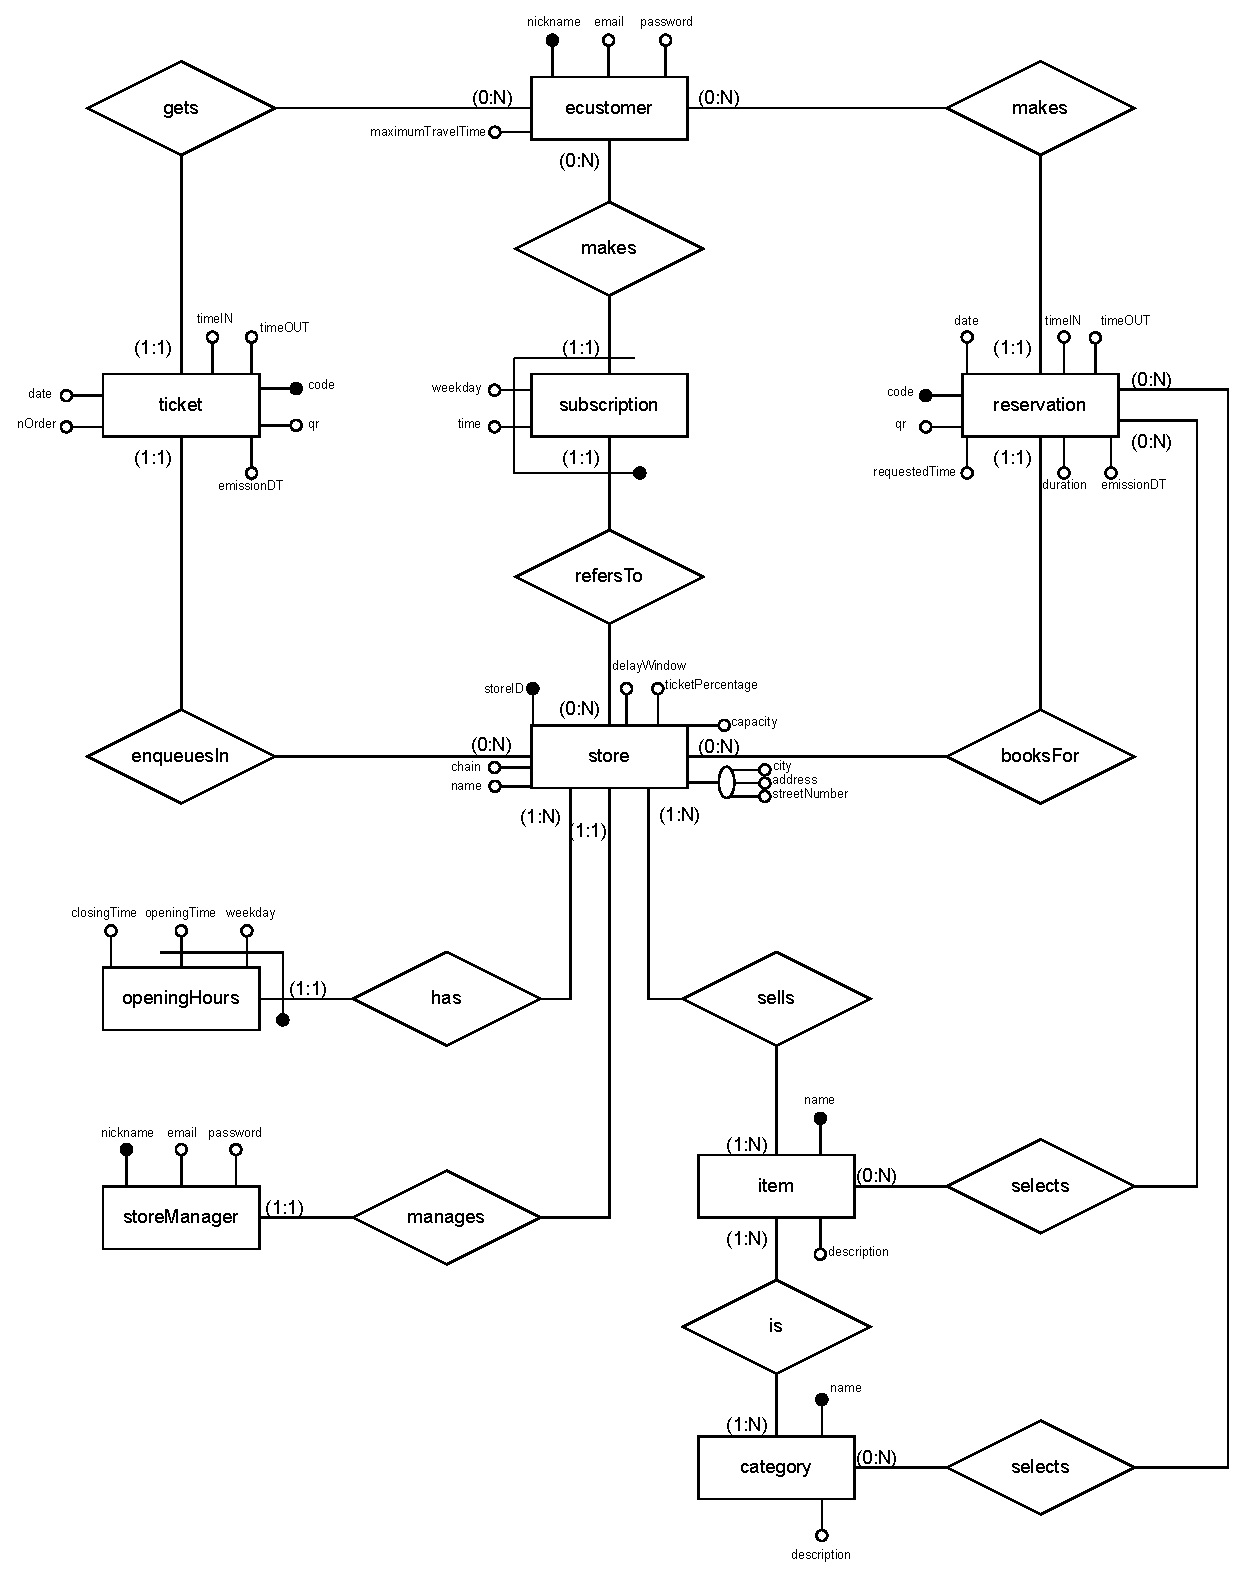
\includegraphics[width=\linewidth] {er_diagram/ERDiagram}
	\caption{ER diagram of the database}
	\label{er} 
\end{figure}
\clearpage
% Component view subsection, to be included in architecture.tex

\subsection{Component view}
This section illustrates the components of the application. Figure \ref{highcomp} offers an high-level representation of the web application's modules; to keep the scheme as clear as possible and avoid modules duplication (which can result misleading), the mobile application module has been omitted, as it connects exactly like the webapp's one. The next sections offer a greater detail on the subsystems, while the components shown here are:

\begin{itemize}[itemsep=-1mm, topsep=-1mm]
	\item Maps Adapter: component used to interface the application with the mapping service's API
	\item Data Access Module: represents the system used to query the relational database 
\end{itemize}

\begin{figure}[h]	
	\centering
	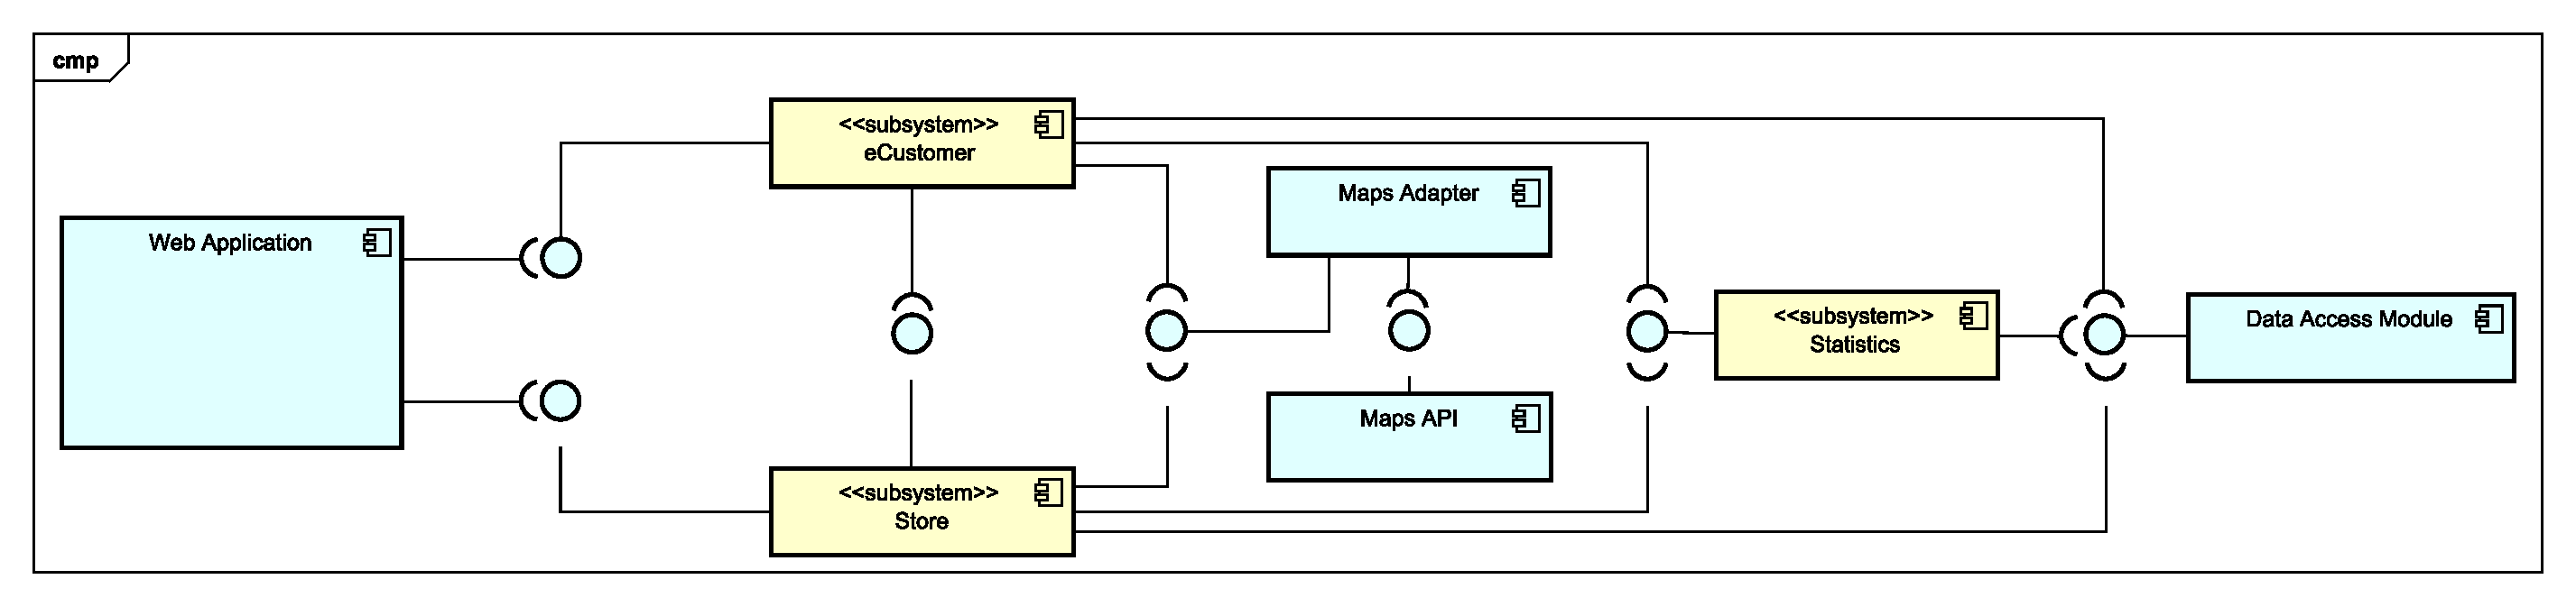
\includegraphics[width=\linewidth] {component_diagrams/component_high}
	\caption{High-level component view}
	\label{highcomp} 
\end{figure}

\subsubsection{Store subsystem}
The store subsystem modules, as shown in Figure 5, are the following:
\begin{itemize}[itemsep=-1mm, topsep=-1mm]
	\item SM Account Manager Module: allows to modify information related to the Store Manager's account
	\item Store Info Manager Module: enables the insert and update of data related to the store (capacity, delay window, items...)
	\item Access Creation Module: controls the creation of reservations and tickets (including the printing of physical ones)
	\item Queue Manager Module: manages a queue of tickets, allowing all operations such as enqueue and dequeue
	\item Visit Manager Module: is responsible for creating visits, scheduling entrances, handle delays, scan codes and manage the customers inside 
\end{itemize}\vspace{.5\baselineskip} 
The connections from components to the Account Manager to check if the Store Manager is logged in are omitted to avoid cluttering, as many modules need to check if the user can access their functions.

\subsubsection{e-Customer subsystem}
The components that realize the e-Customer subsystem are shown in Figure \ref{ecc}. They are:
\begin{itemize}[itemsep=-1mm, topsep=-1mm]
	\item eC Account Manager Module: allows the modification of the e-Customer's profile
	\item Store Recommender Module: manages the retrieval and proposal of stores to the e-Customer; considers location, travel time and store state to create its lists
	\item Access Request Module: is the module responsible for requesting the creation of tickets and reservations and handles the user interaction
	\item Requests Manager Module: controls the visualization and deletion of active tickets and reservations
	\item Notification Module: sends all notifications to the e-Customer when requested by other modules
	\item Subscription Module: handles the user's requests for slot notifications 
\end{itemize}\vspace{.5\baselineskip} 
Internal connections to the Account Manager used to check if the e-Customer is logged in are omitted.

\begin{figure}[p]	
	\centering
	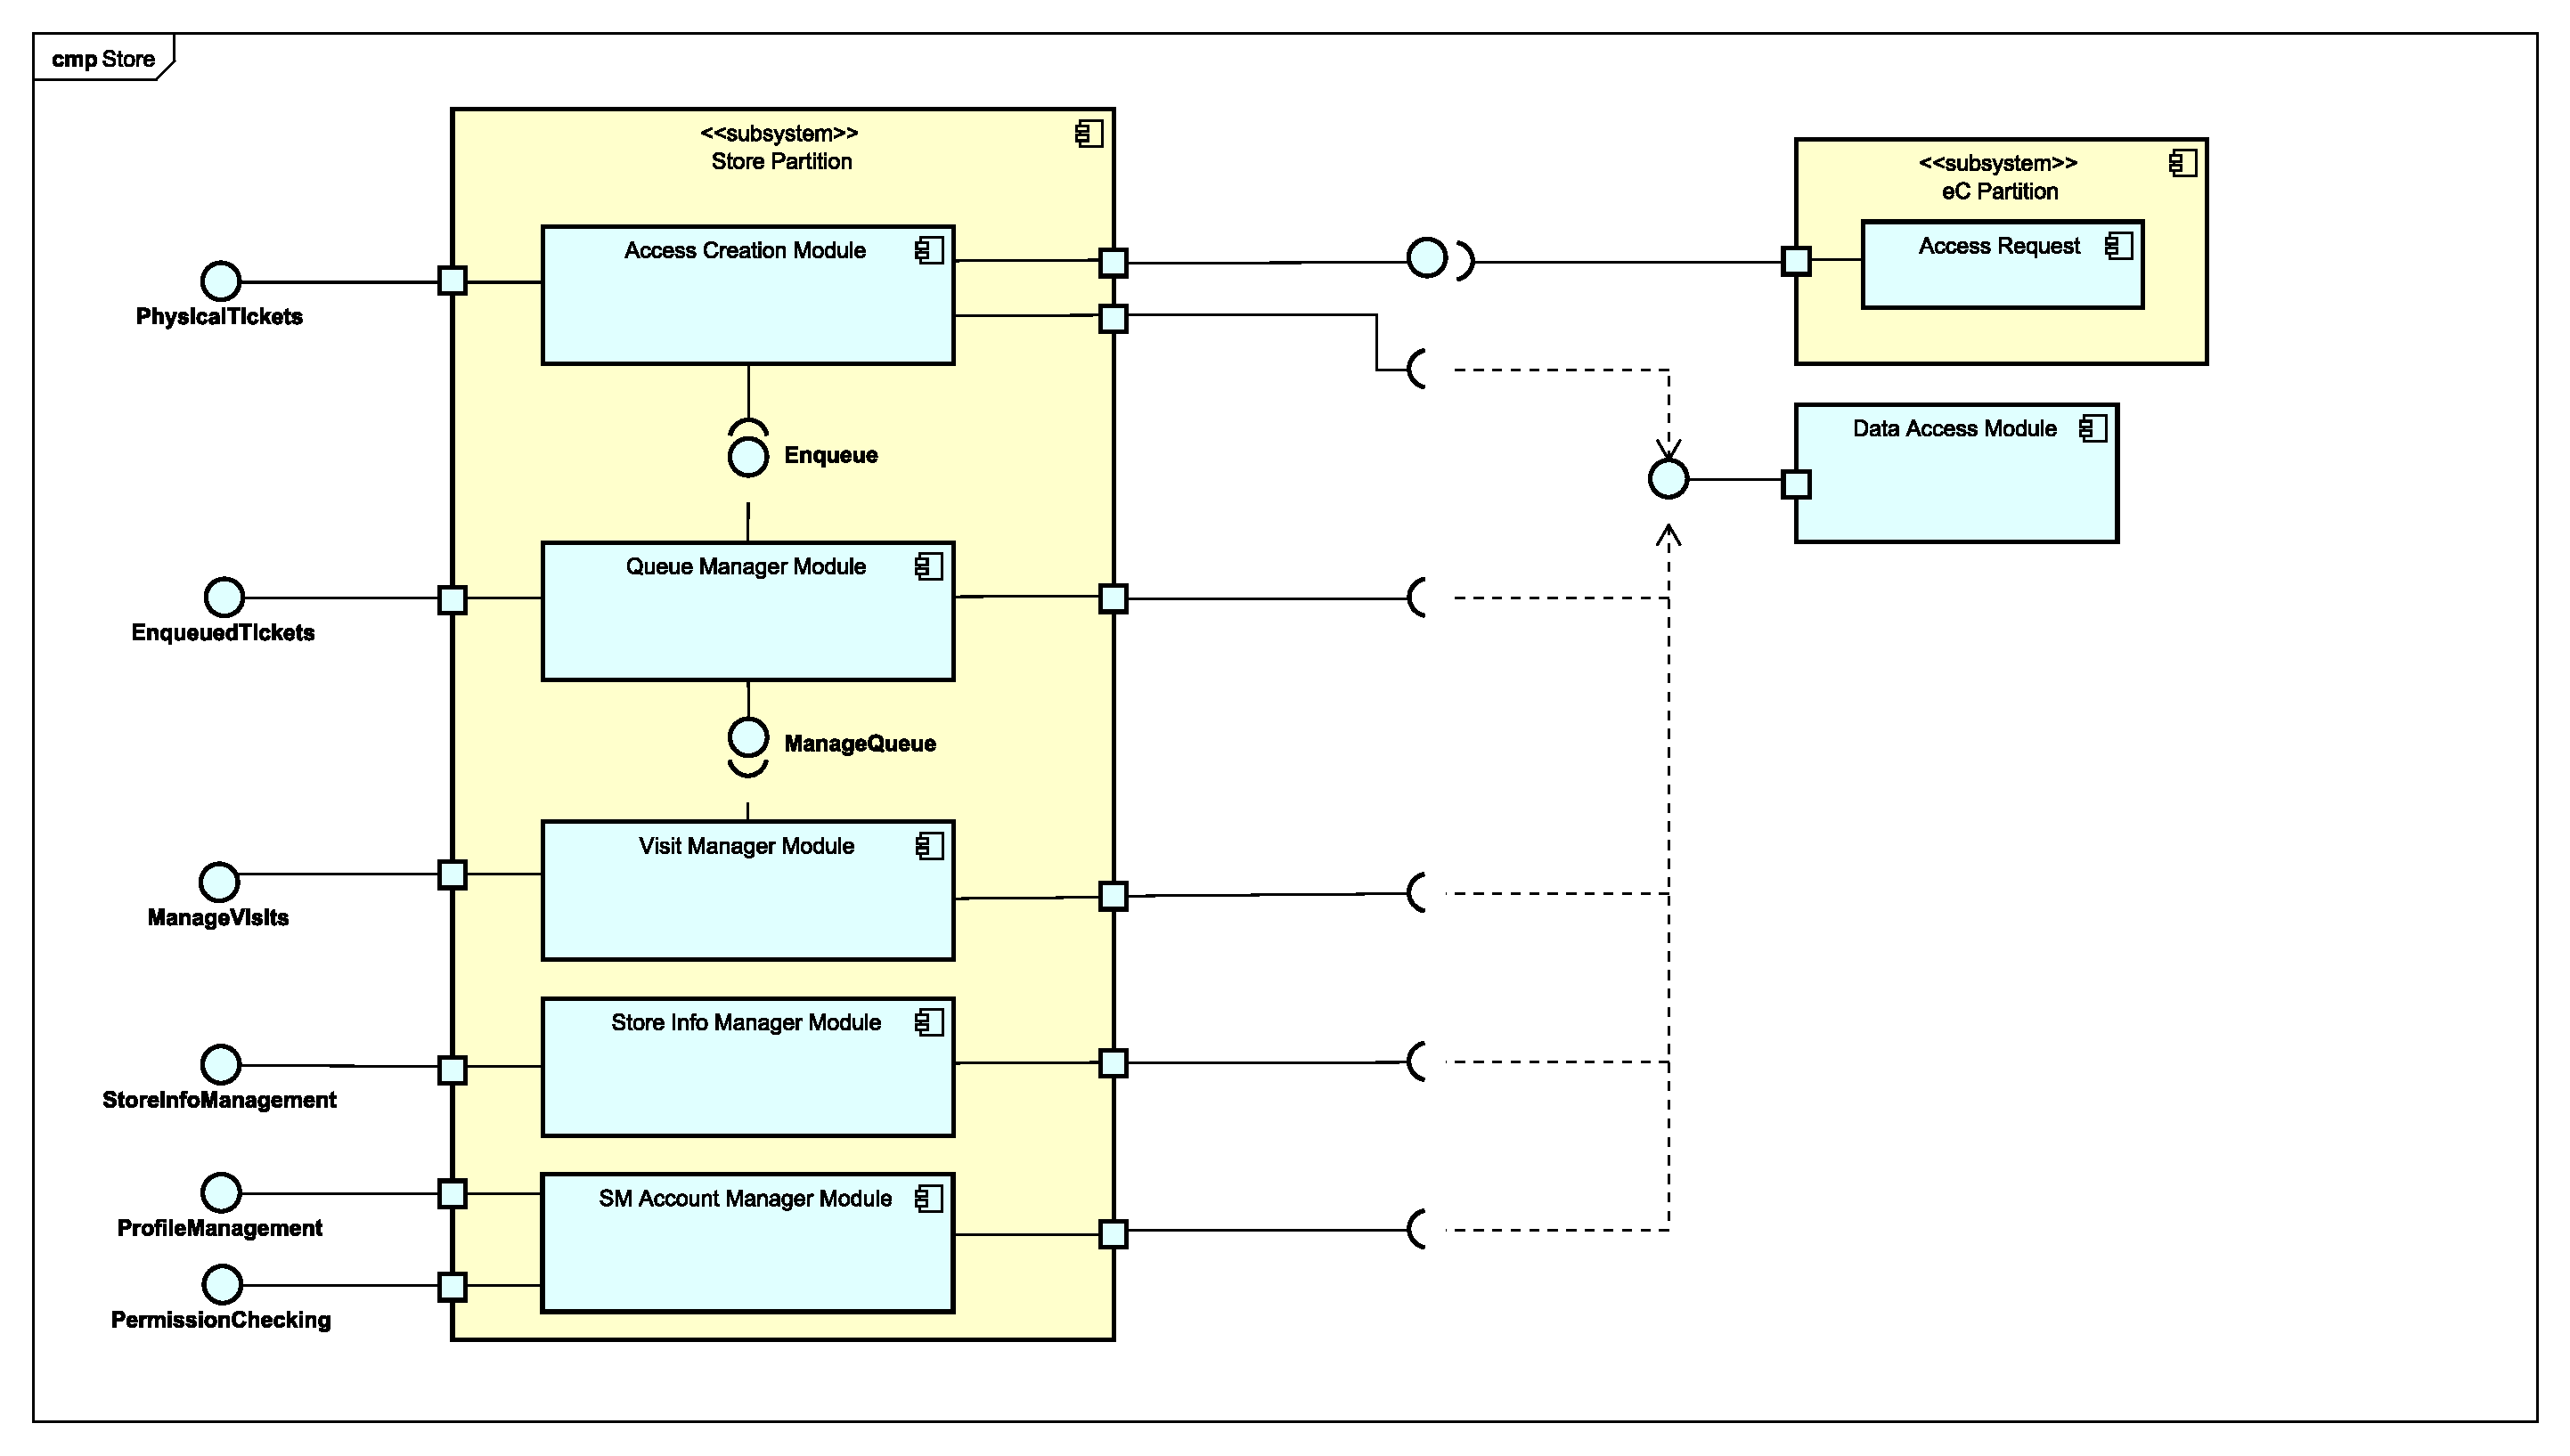
\includegraphics[width=\linewidth] {component_diagrams/component_store}
	\caption{Component view of the Store Manager subsystem}
	\label{smc} 
	
	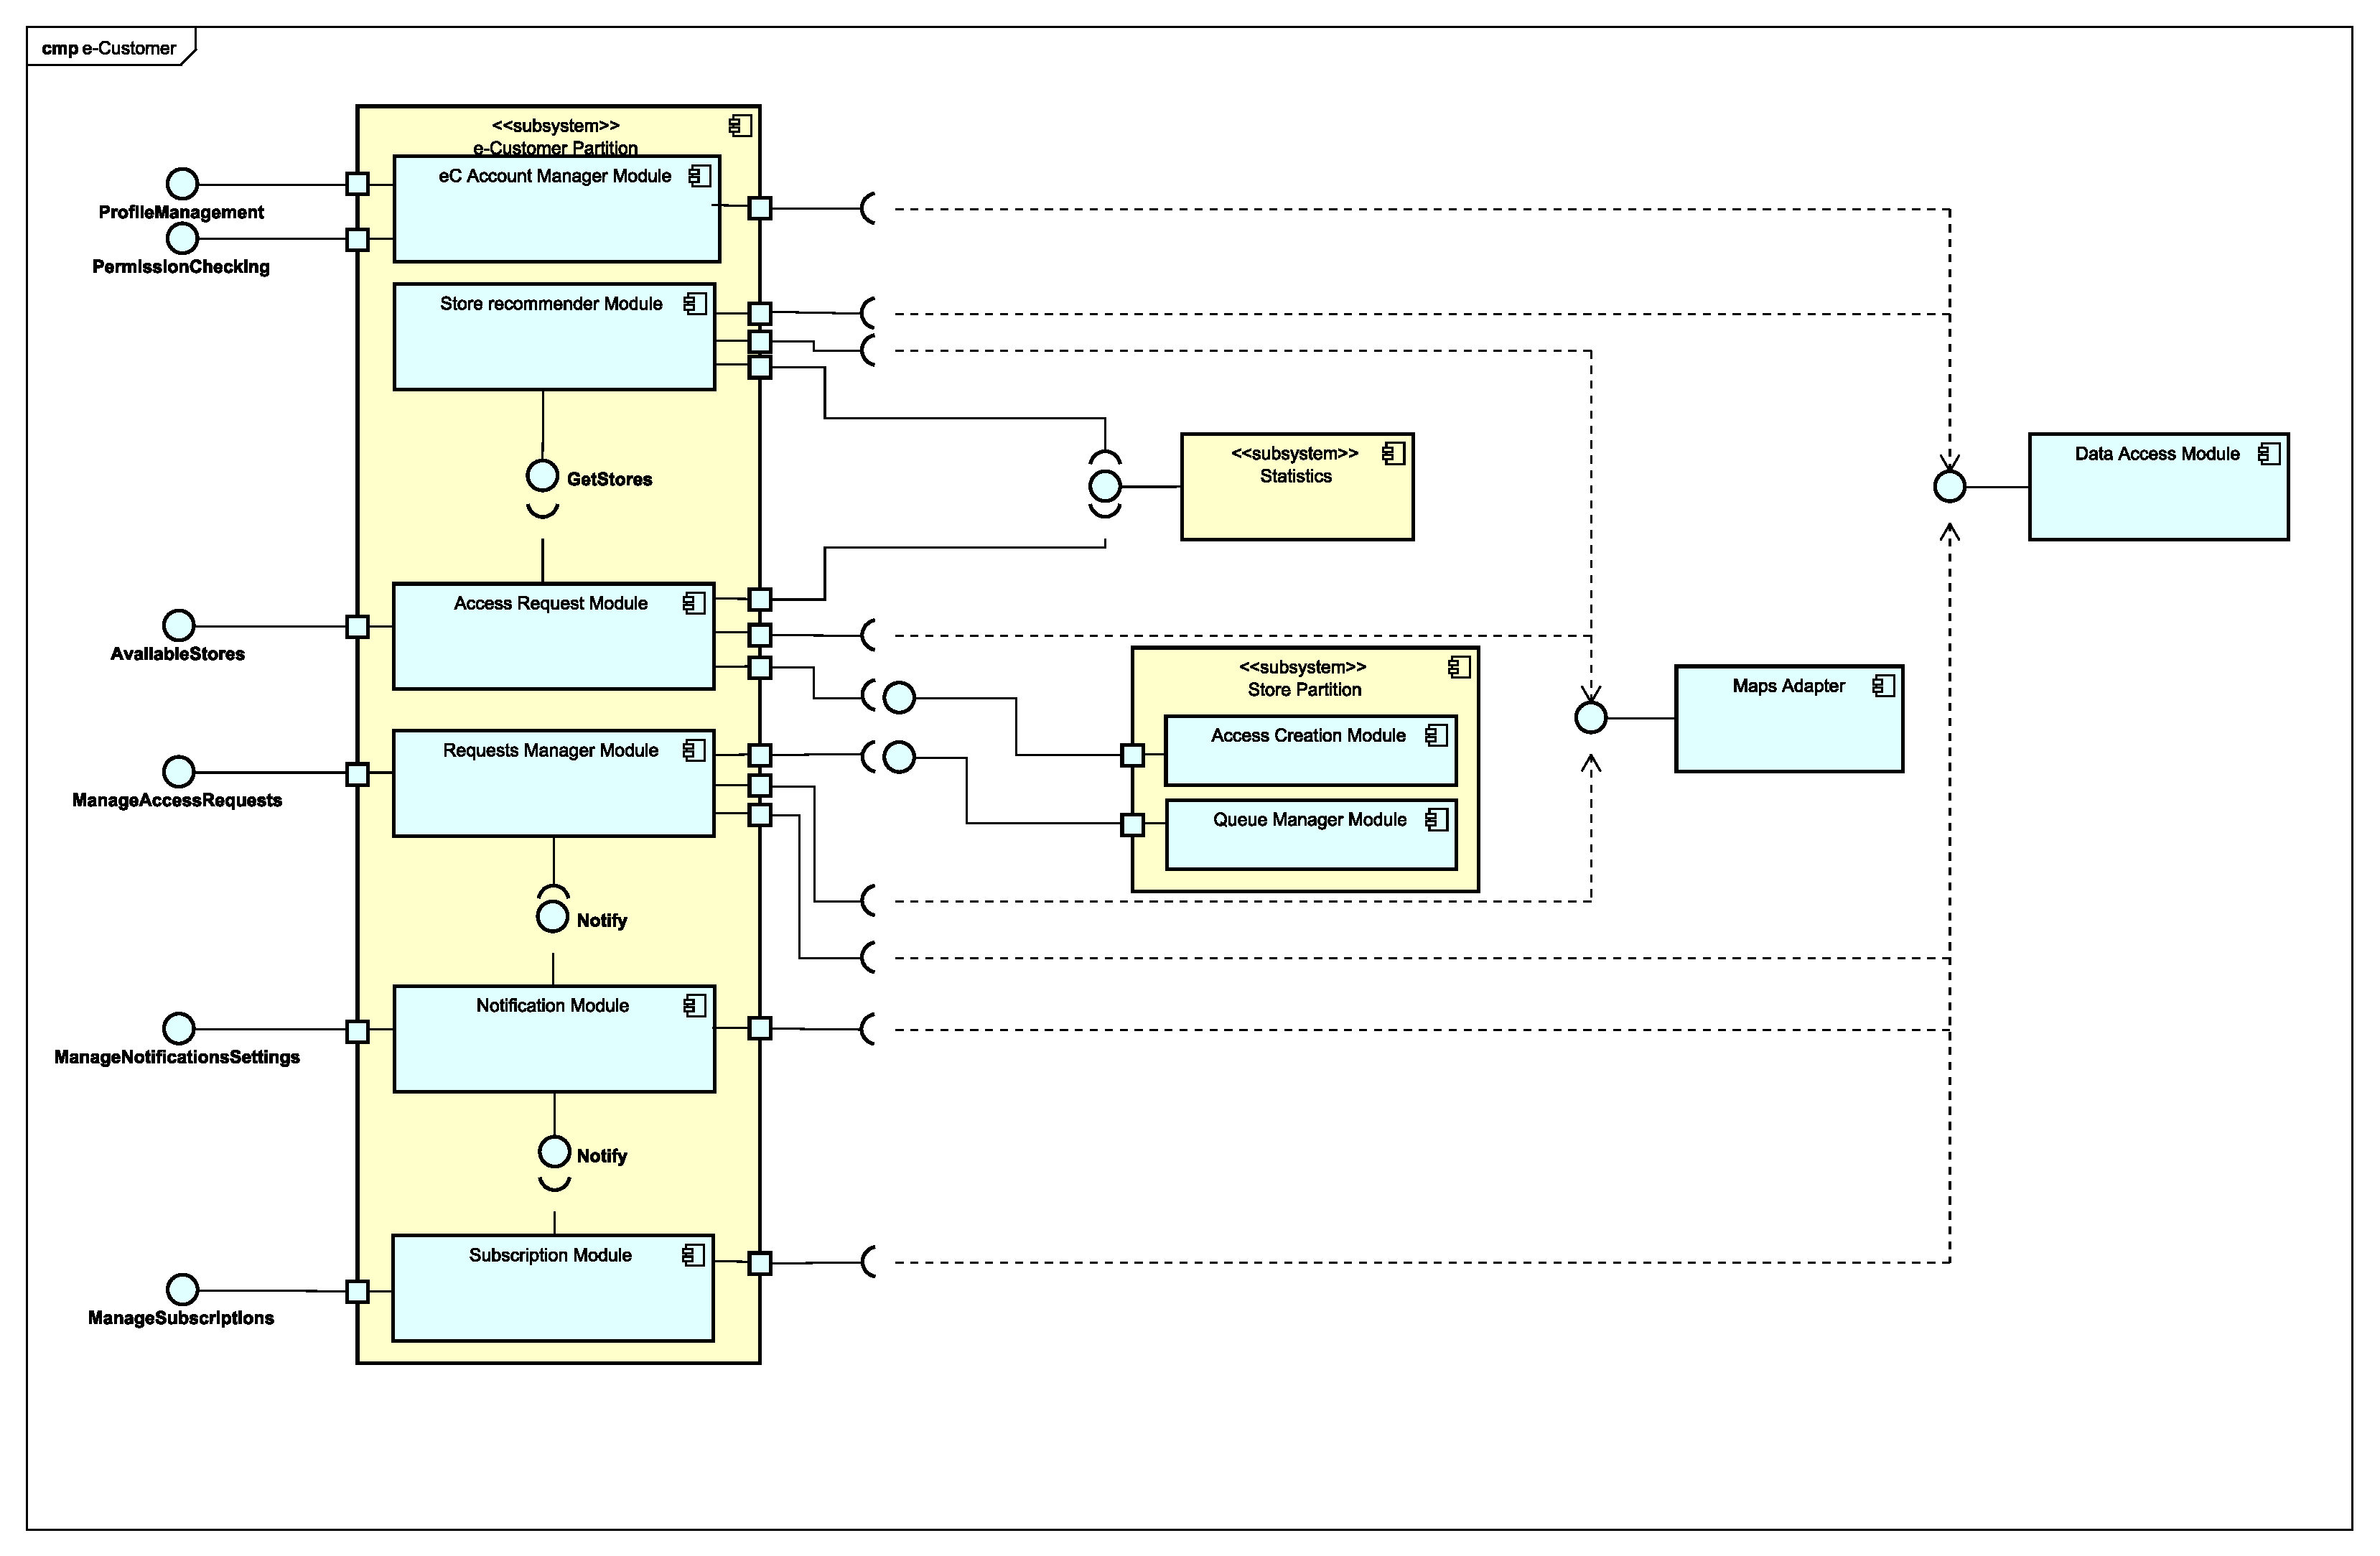
\includegraphics[width=\linewidth] {component_diagrams/component_eC}
	\caption{Component view of the e-Customer subsystem}
	\label{ecc} 
\end{figure}

\subsubsection{Statistics subsystem}
The Statistics subsystem is shown in Figure \ref{stats}. It is composed of:
\begin{itemize}[itemsep=-1mm, topsep=-1mm]
	\item Customer statistics: is responsible for elaborating data such as visit time or preferred store
	\item Store statistics: computes and aggregates data like average time of visit or mean time of queue
\end{itemize}

\begin{figure}[h]	
	\centering
	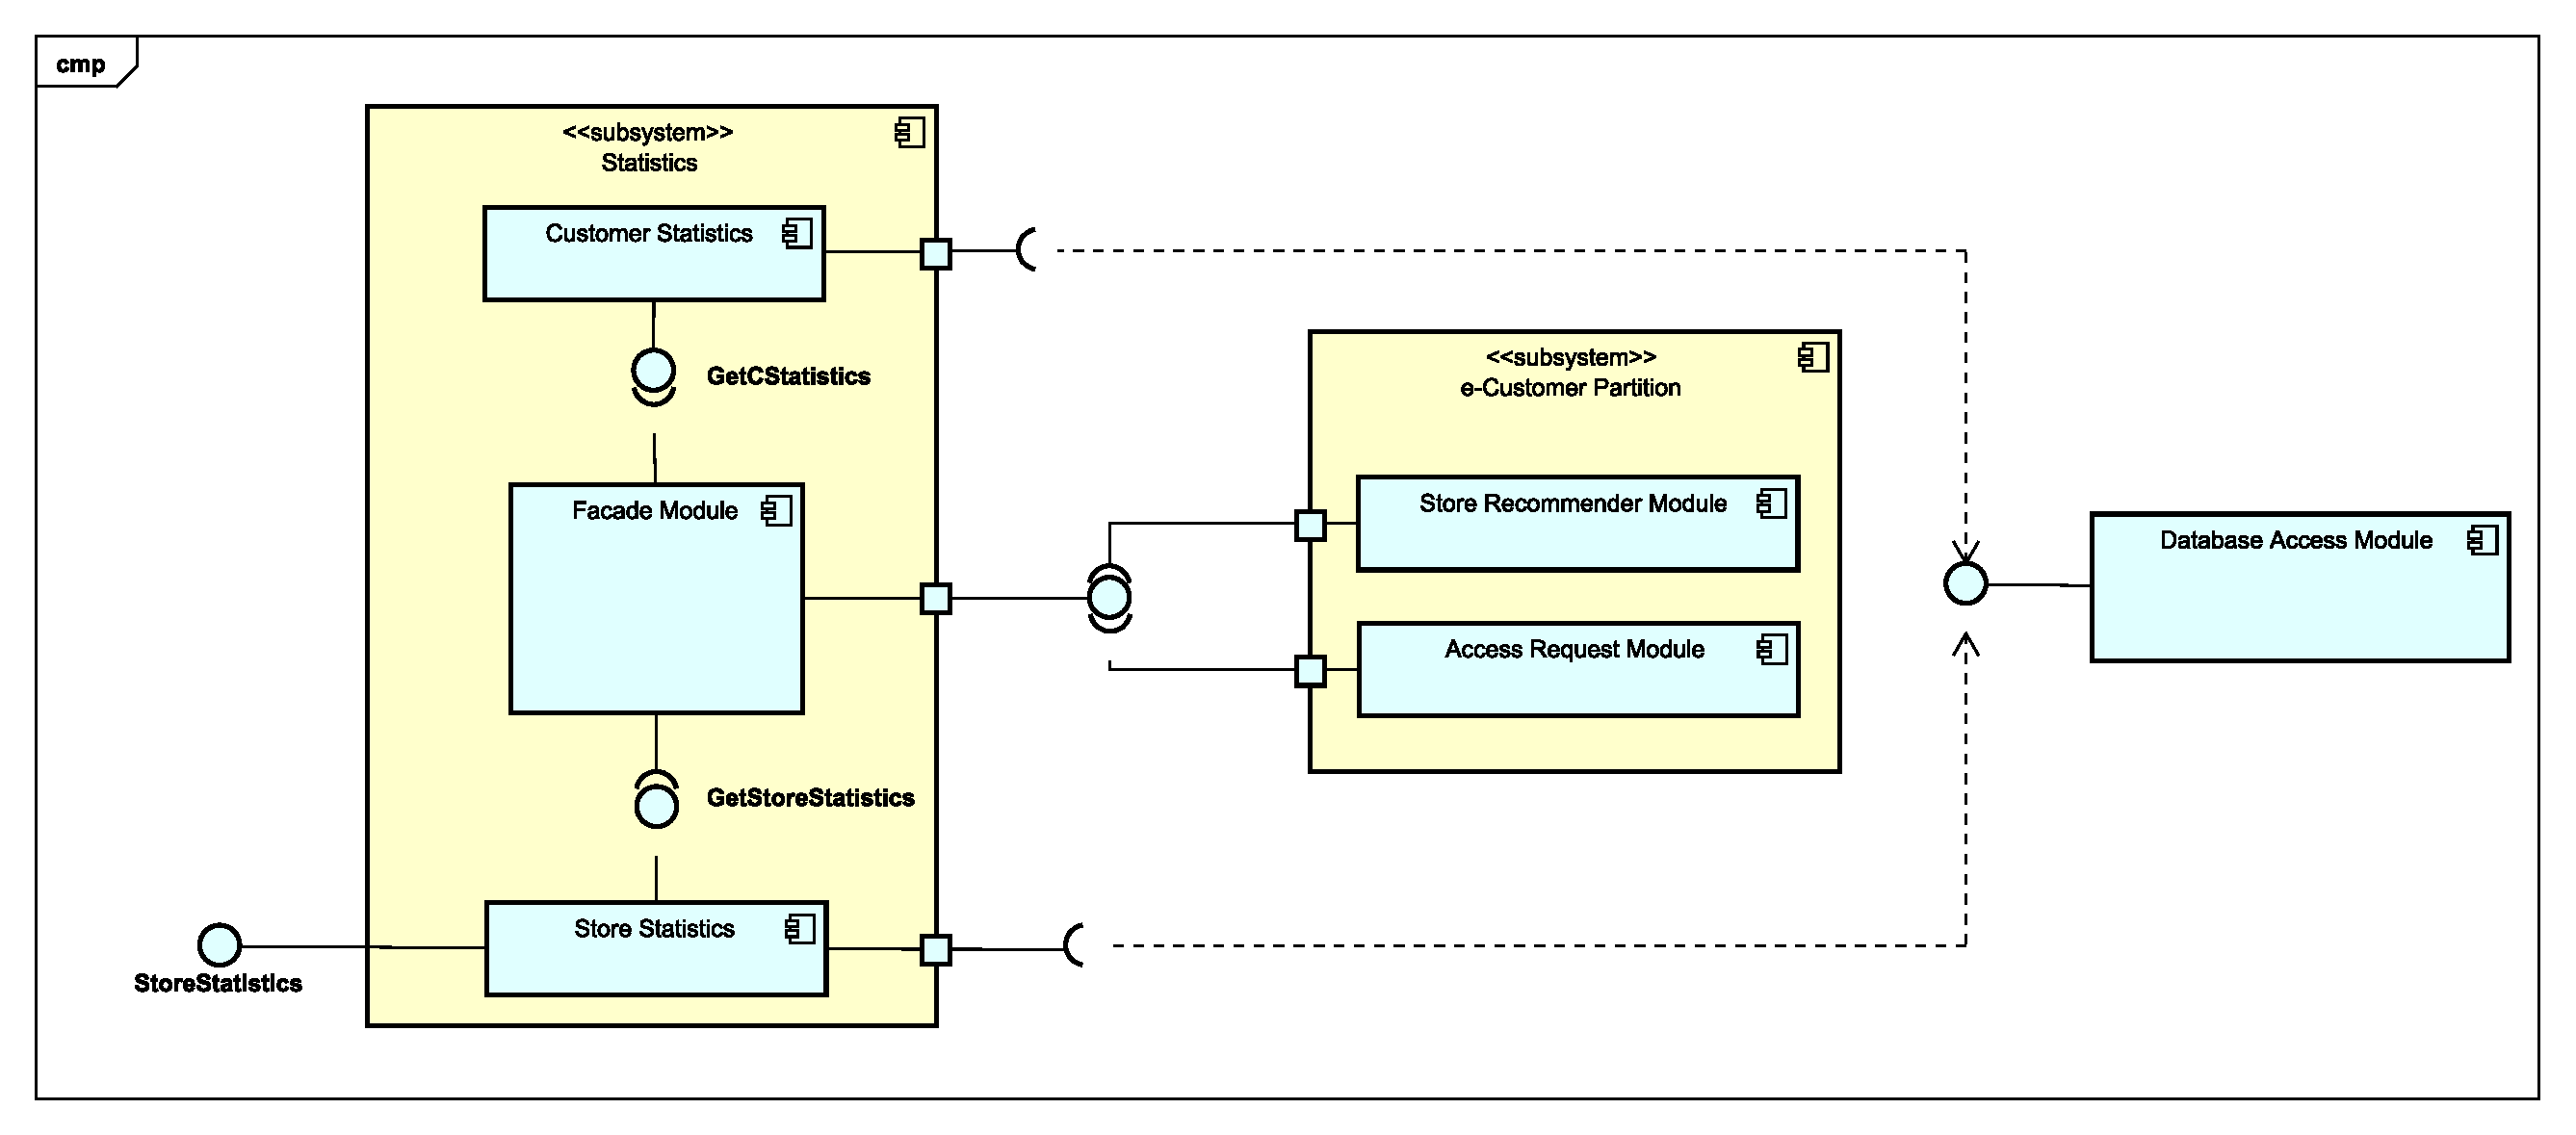
\includegraphics[width=\linewidth] {component_diagrams/statistics}
	\caption{Component view of the Statistic subsystem}
	\label{stats} 
\end{figure}

% Deployment view subsection, to be included in architecture.tex

\subsection{Deployment view}
\label{sect:deploy}
The deployment view of the application can be seen in Figure \ref{deploy}. 
It uses a 5-tier architecture to separate the web aspects from the application itself and from the data. This way, the code can be better decomposed to increase reusability and for security reasons, exposing only the web tier to browsers. The safety of the system is ensured by the use of two DMZs, one isolating the web tier from the rest and one to better protect the data layer. 

With respect to the theoretical layer subdivision, layers 2 and 3 have been united through the use of Apache Tomcat, that covers both the web server's and servlet container's functions.

\begin{landscape}
	\begin{figure}[p]
		\centering	
		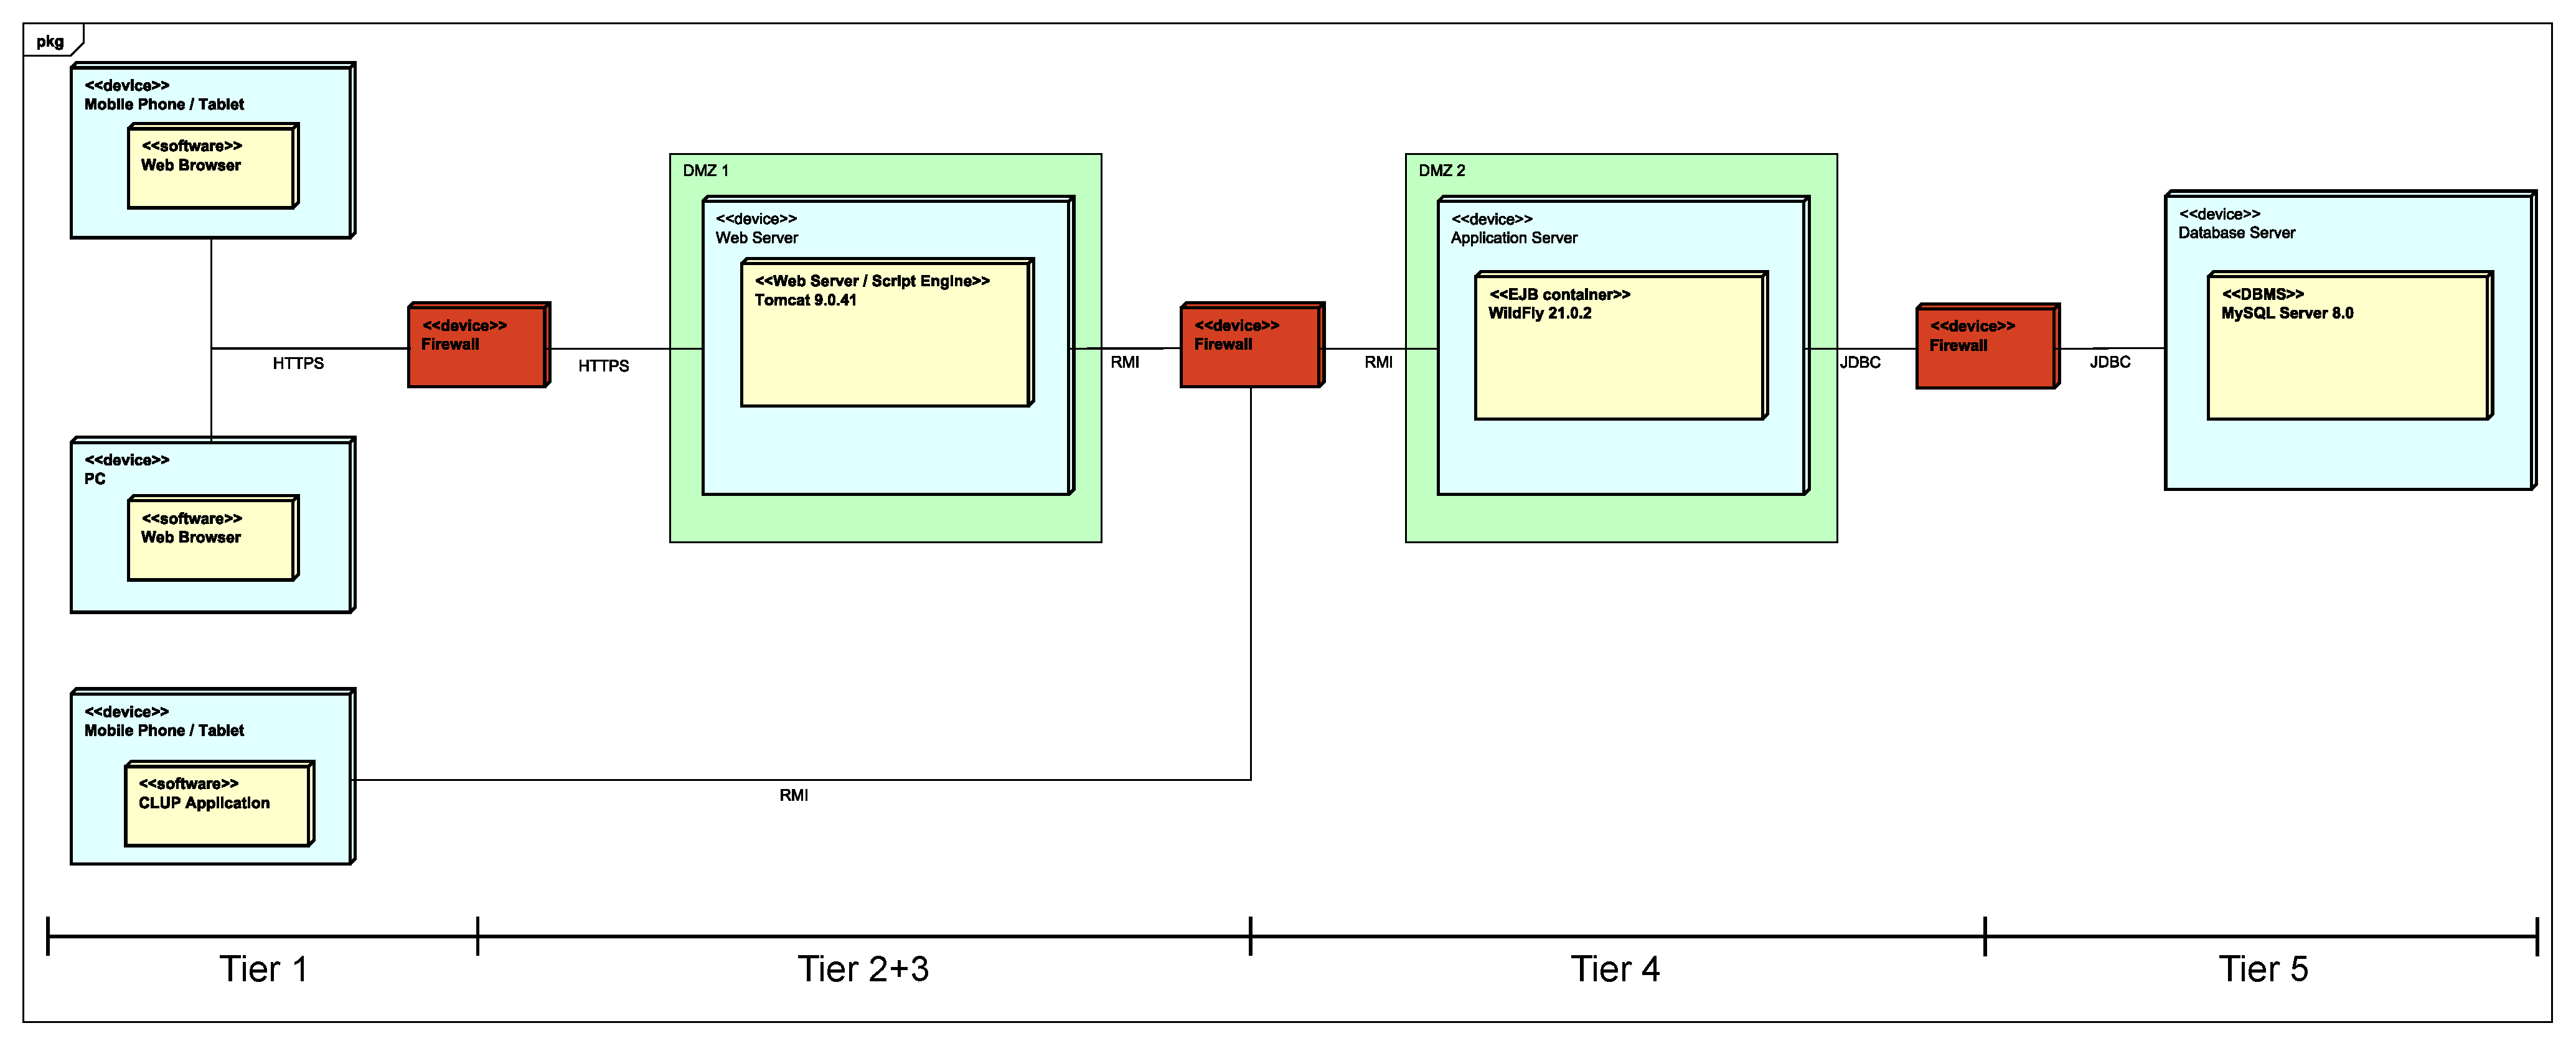
\includegraphics[width=\linewidth] {deployment_diagrams/deployment}
		\caption{Deployment diagram of the application}
		\label{deploy} 
	\end{figure}
\end{landscape}

% Runtime view subsection, to be included in architecture.tex

\subsection{Runtime view}
This section covers some of the interactions among the system's components. 

Figure \ref{runeclogin} shows the interaction between modules to achieve the e-Customer login function.

Diagrams in Figures \ref{runecticket} and \ref{runecvisit} represent the different steps needed for getting a ticket or booking a visit for an e-Customer. The core of these processes is the retrieval of stores, done through the following steps:
\begin{itemize}[itemsep=-1mm, topsep=-1mm]
  	\item The Access Request module asks for the localization of the user
  	\item The Store Recommender requests stores close to the user based on the parameters defined by the user (as mean of transport, maximum travel time...)
  	\item The Recommender then queries the database to know which of the candidate stores use CLup
  	\item The returned stores are checked for availability to host more tickets based on the queues and time of visits
  	\item The finally filtered list is then returned to the user
\end{itemize}\vspace{.5\baselineskip}
This order has been defined to offer an incremental filter, allowing to access the maps API only once and limit the accesses to the DB to requests only for previously identified store. Furthermore, the request for stores on a geographic base would be limited anyway even for large cities\textsuperscript{\cite{food}}, as opposed to extracting all stores in the database.

\begin{figure}[h]	
	\centering
	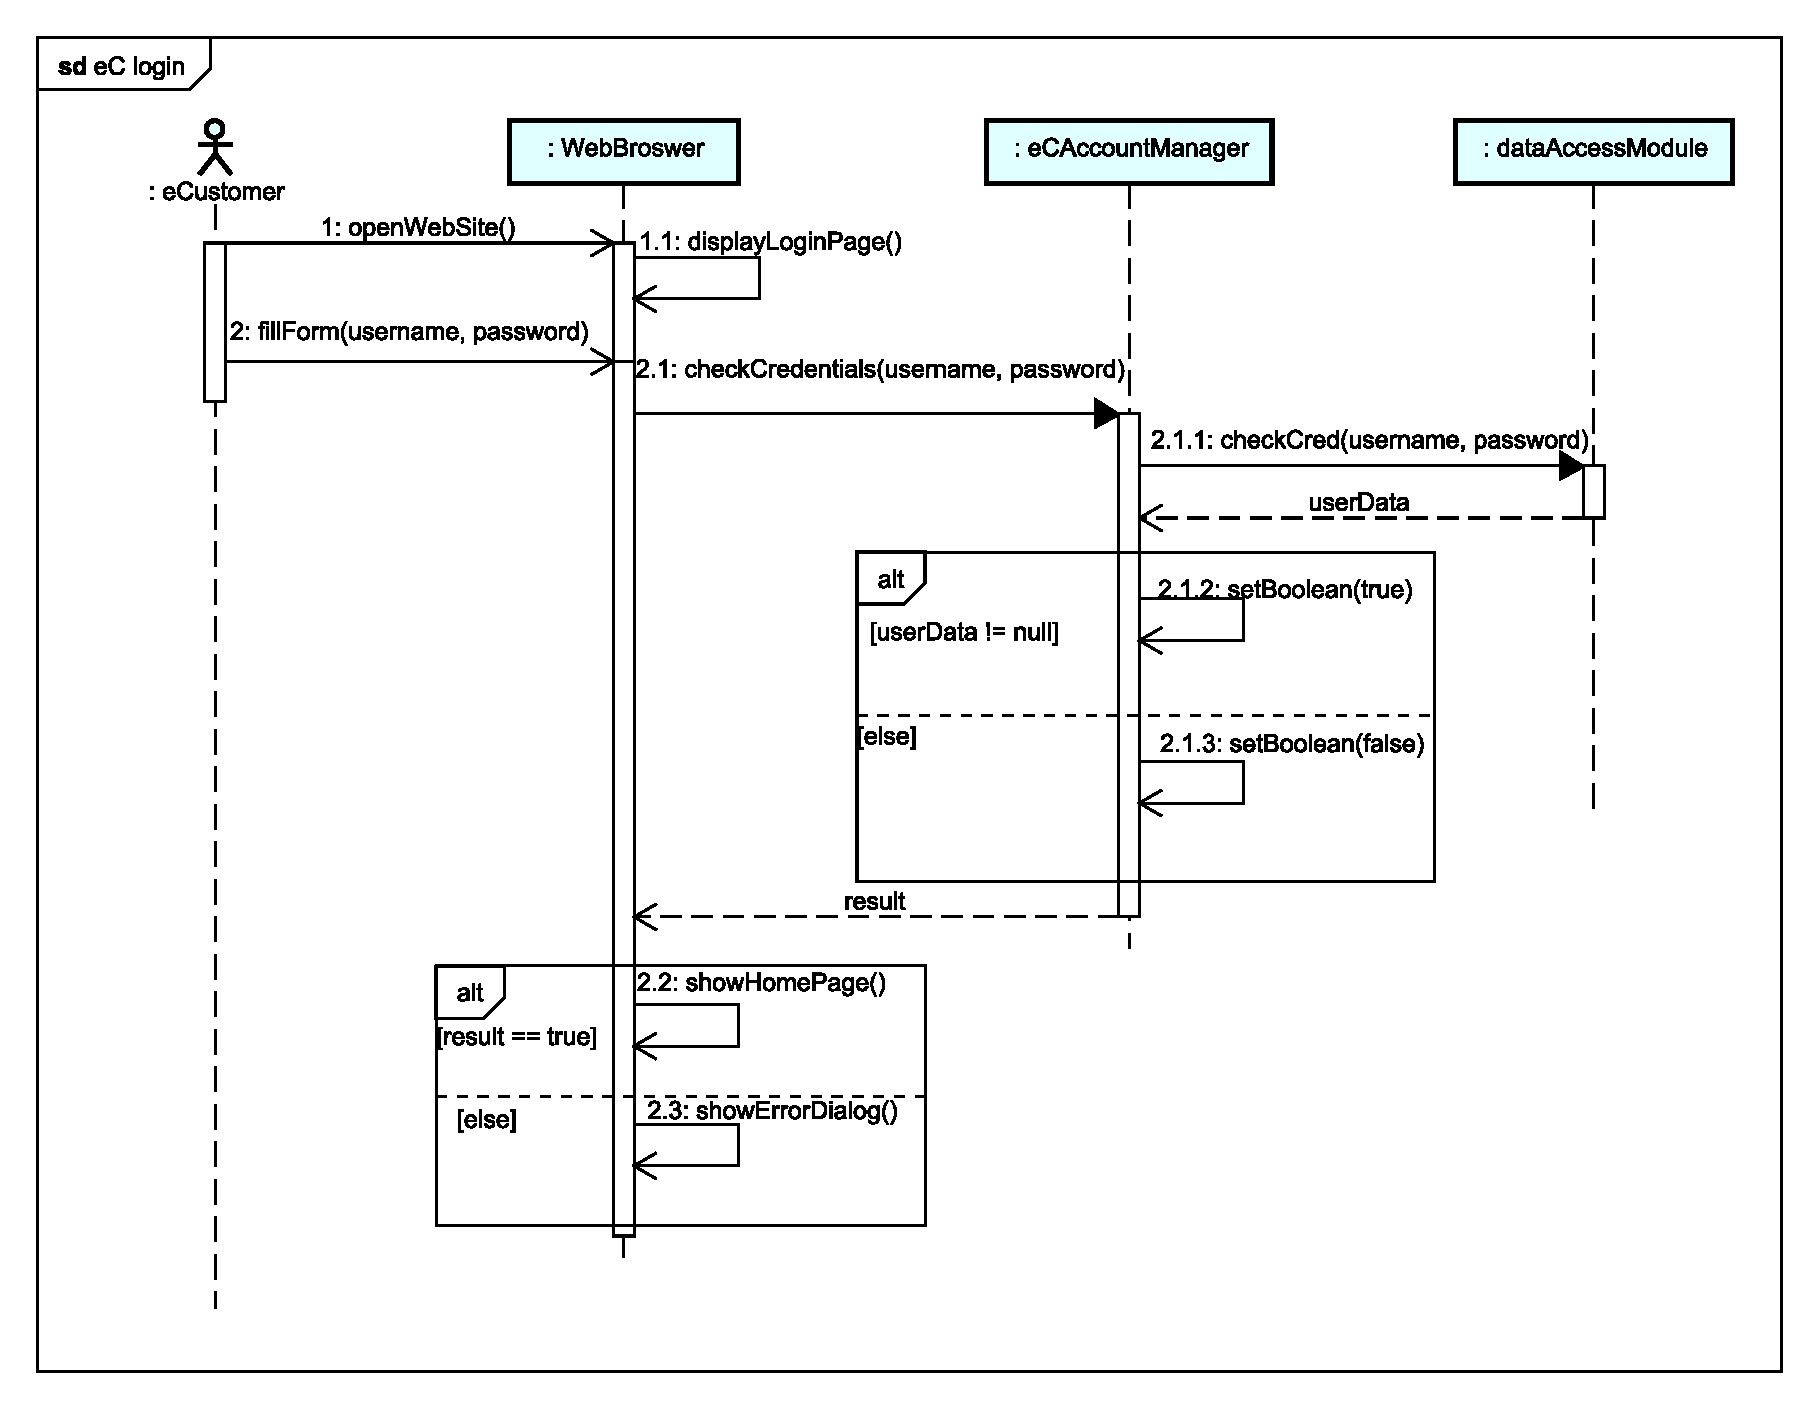
\includegraphics[width=\linewidth] {sequence_diagrams/eC_login_seqD}
	\caption{Runtime view of an e-Customer login}
	\label{runeclogin} 
\end{figure}

\begin{landscape}
	\begin{figure}[p]
		\centering	
		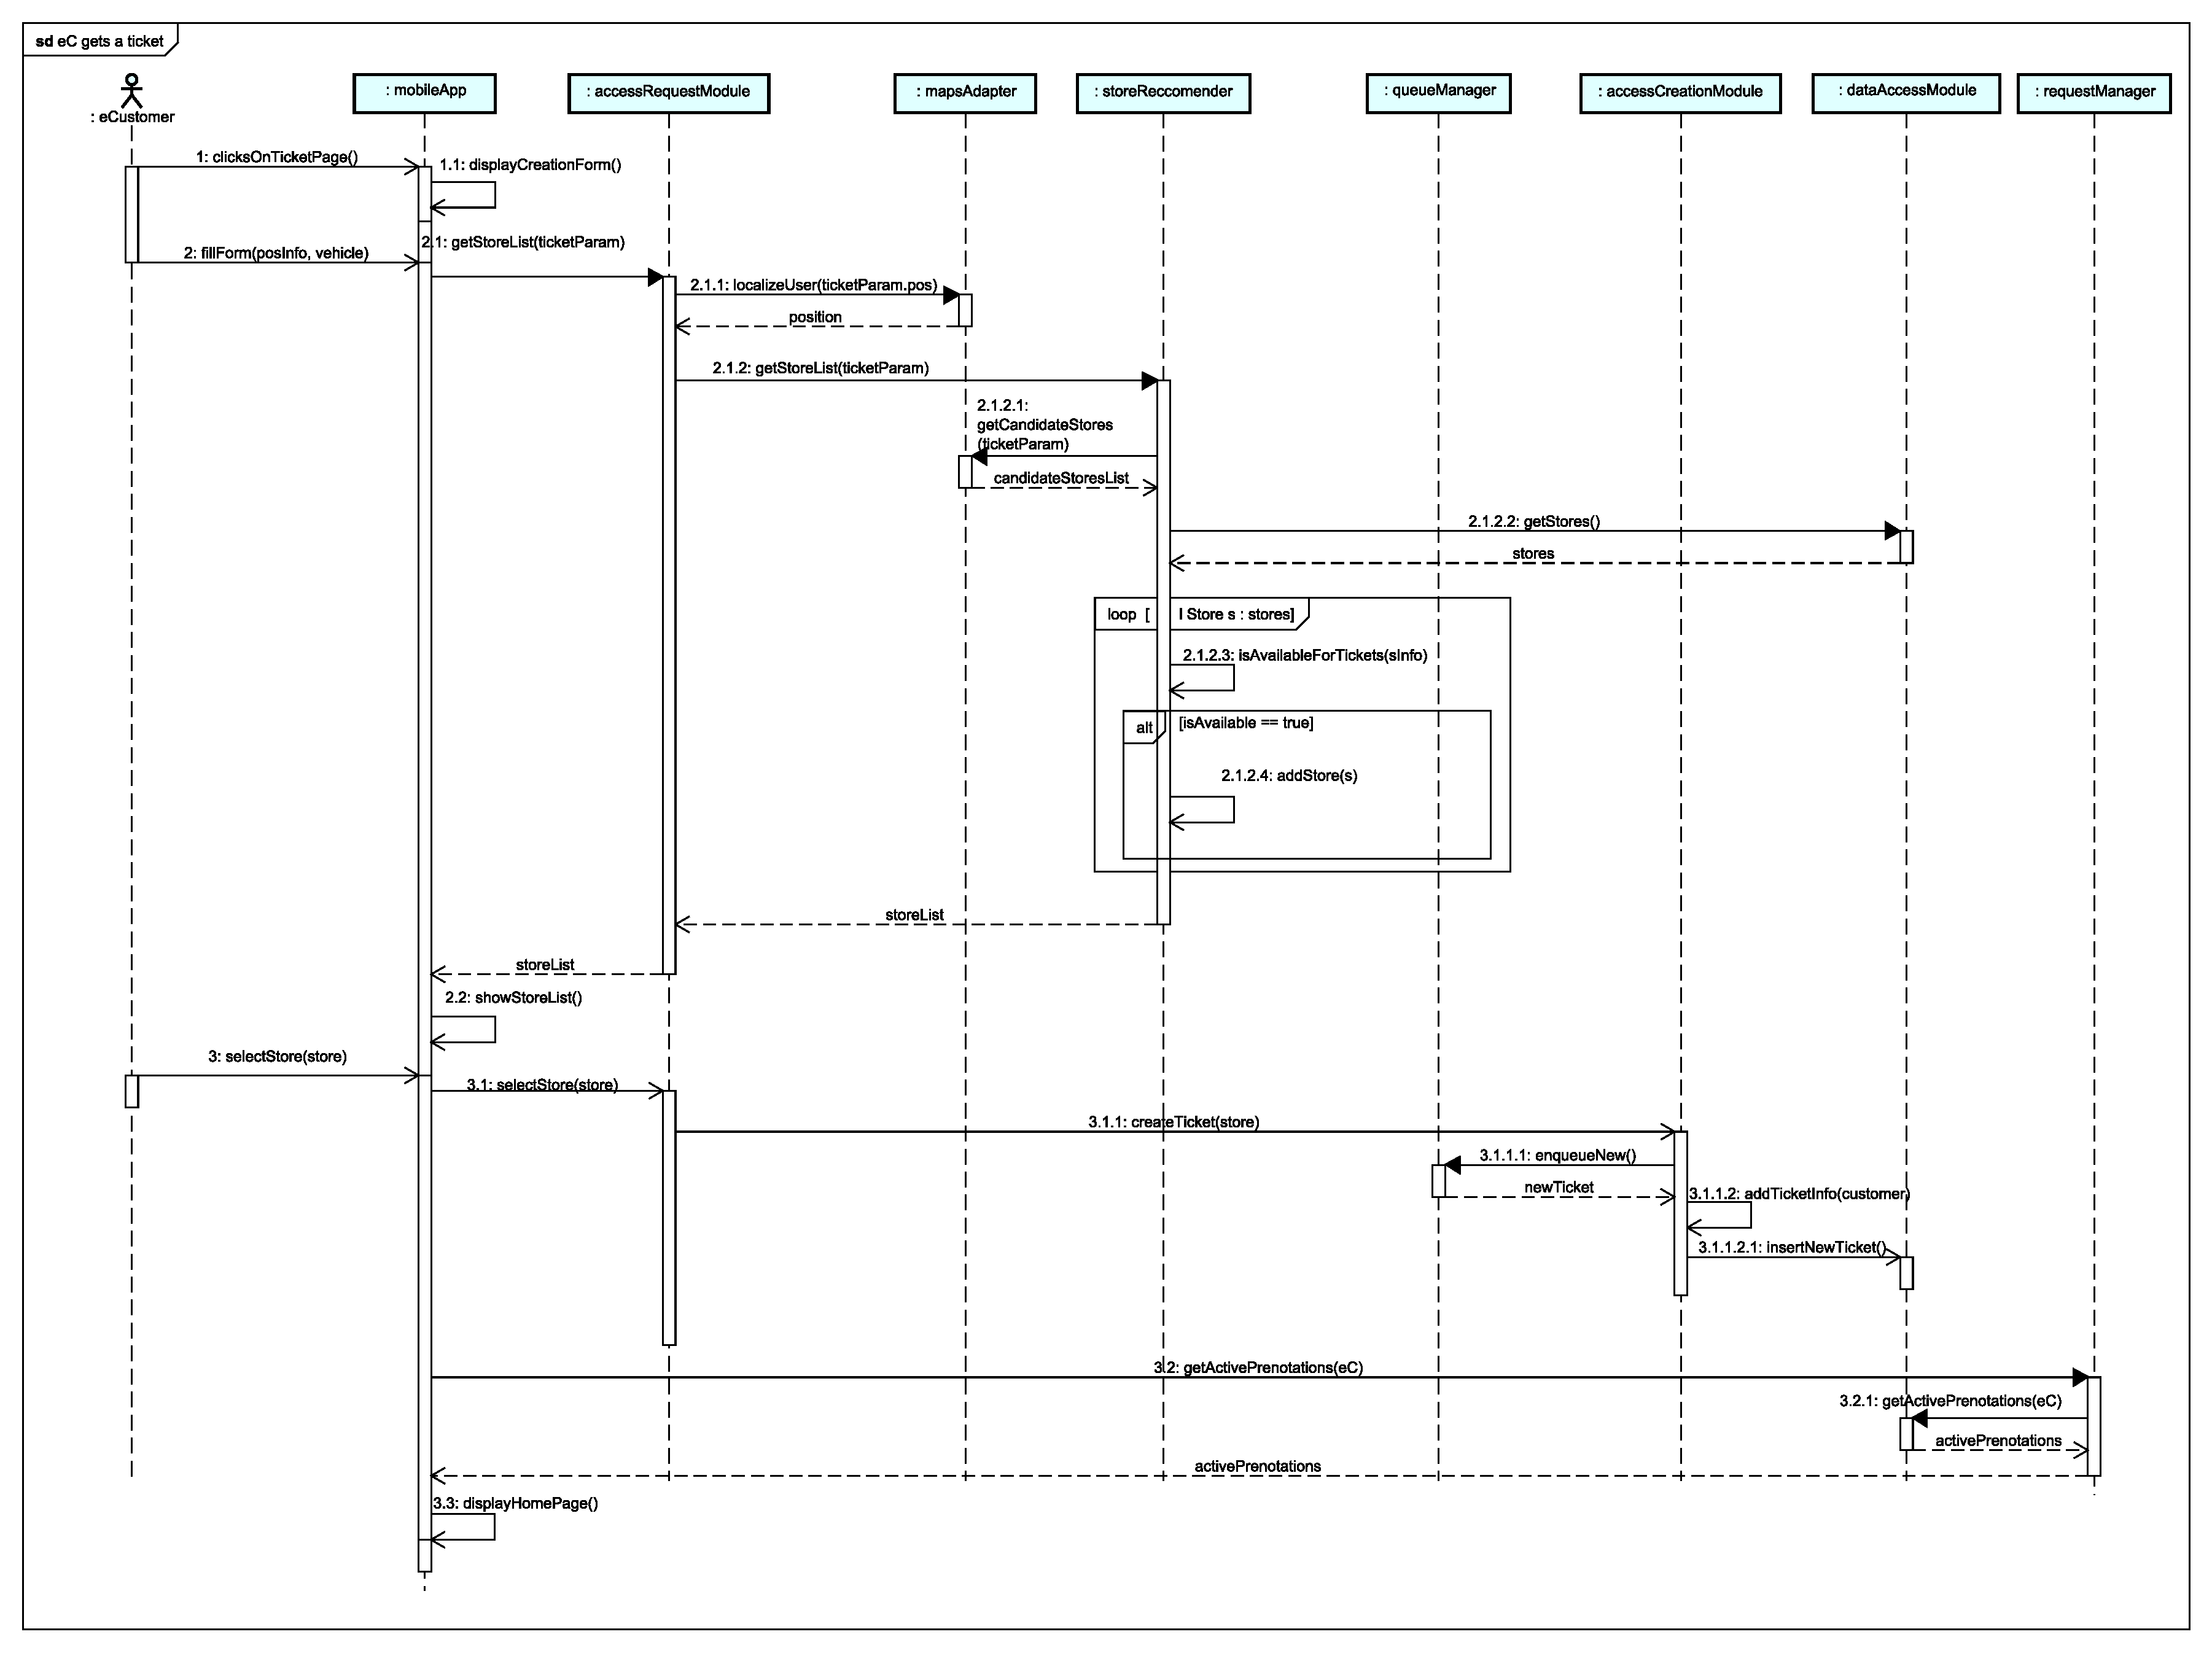
\includegraphics[height=\textheight] {sequence_diagrams/eC_gets_a_ticket_seqD}
		\caption{Runtime view of an e-Customer getting a ticket}
		\label{runecticket} 
	\end{figure}
	
	\begin{figure}[p]
		\centering	
		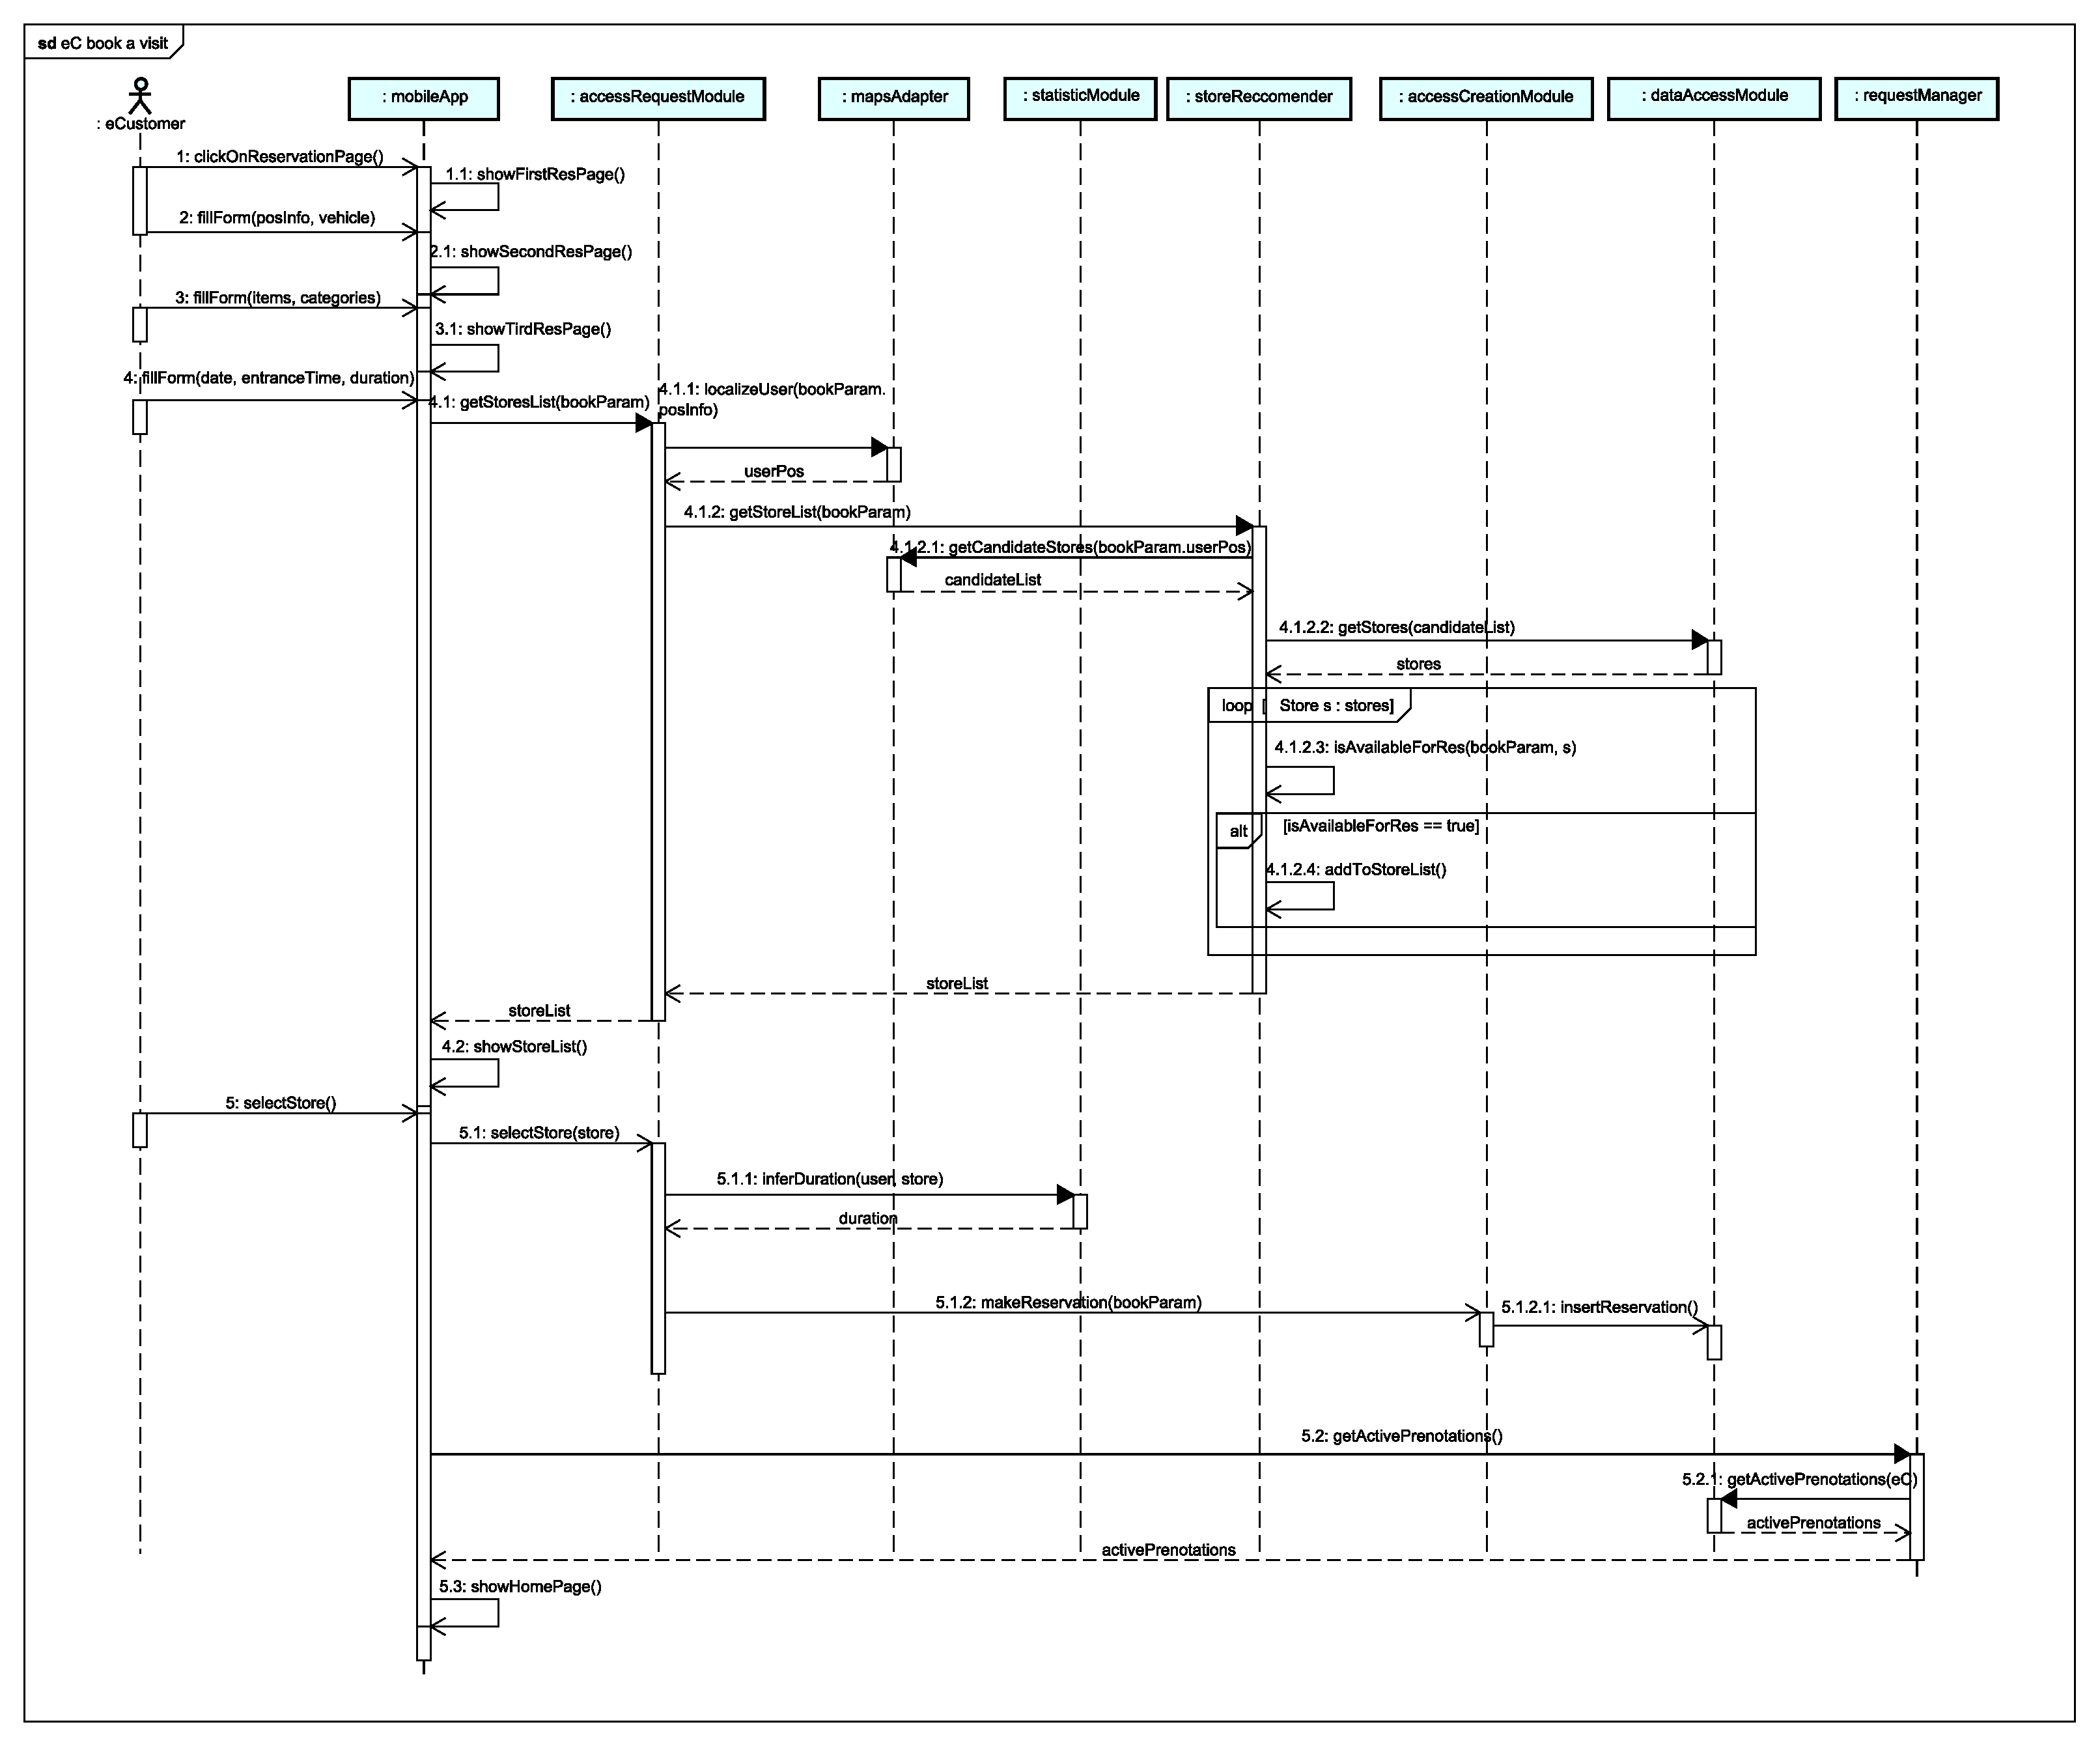
\includegraphics[height=\textheight] {sequence_diagrams/eC_book_a_visit_seqD}
		\caption{Runtime view of an e-Customer booking a visit}
		\label{runecvisit} 
	\end{figure}
\end{landscape}


Figure \ref{ecdelete} illustrates how the request of ticket deletion by an e-Customer is carried out, while Figures \ref{smmodinfo} and \ref{runsmmonitor} concern Store Manager activities, namely modifying their store's information and scanning entering tickets or reservations.

\begin{figure}[h]	
	\centering
	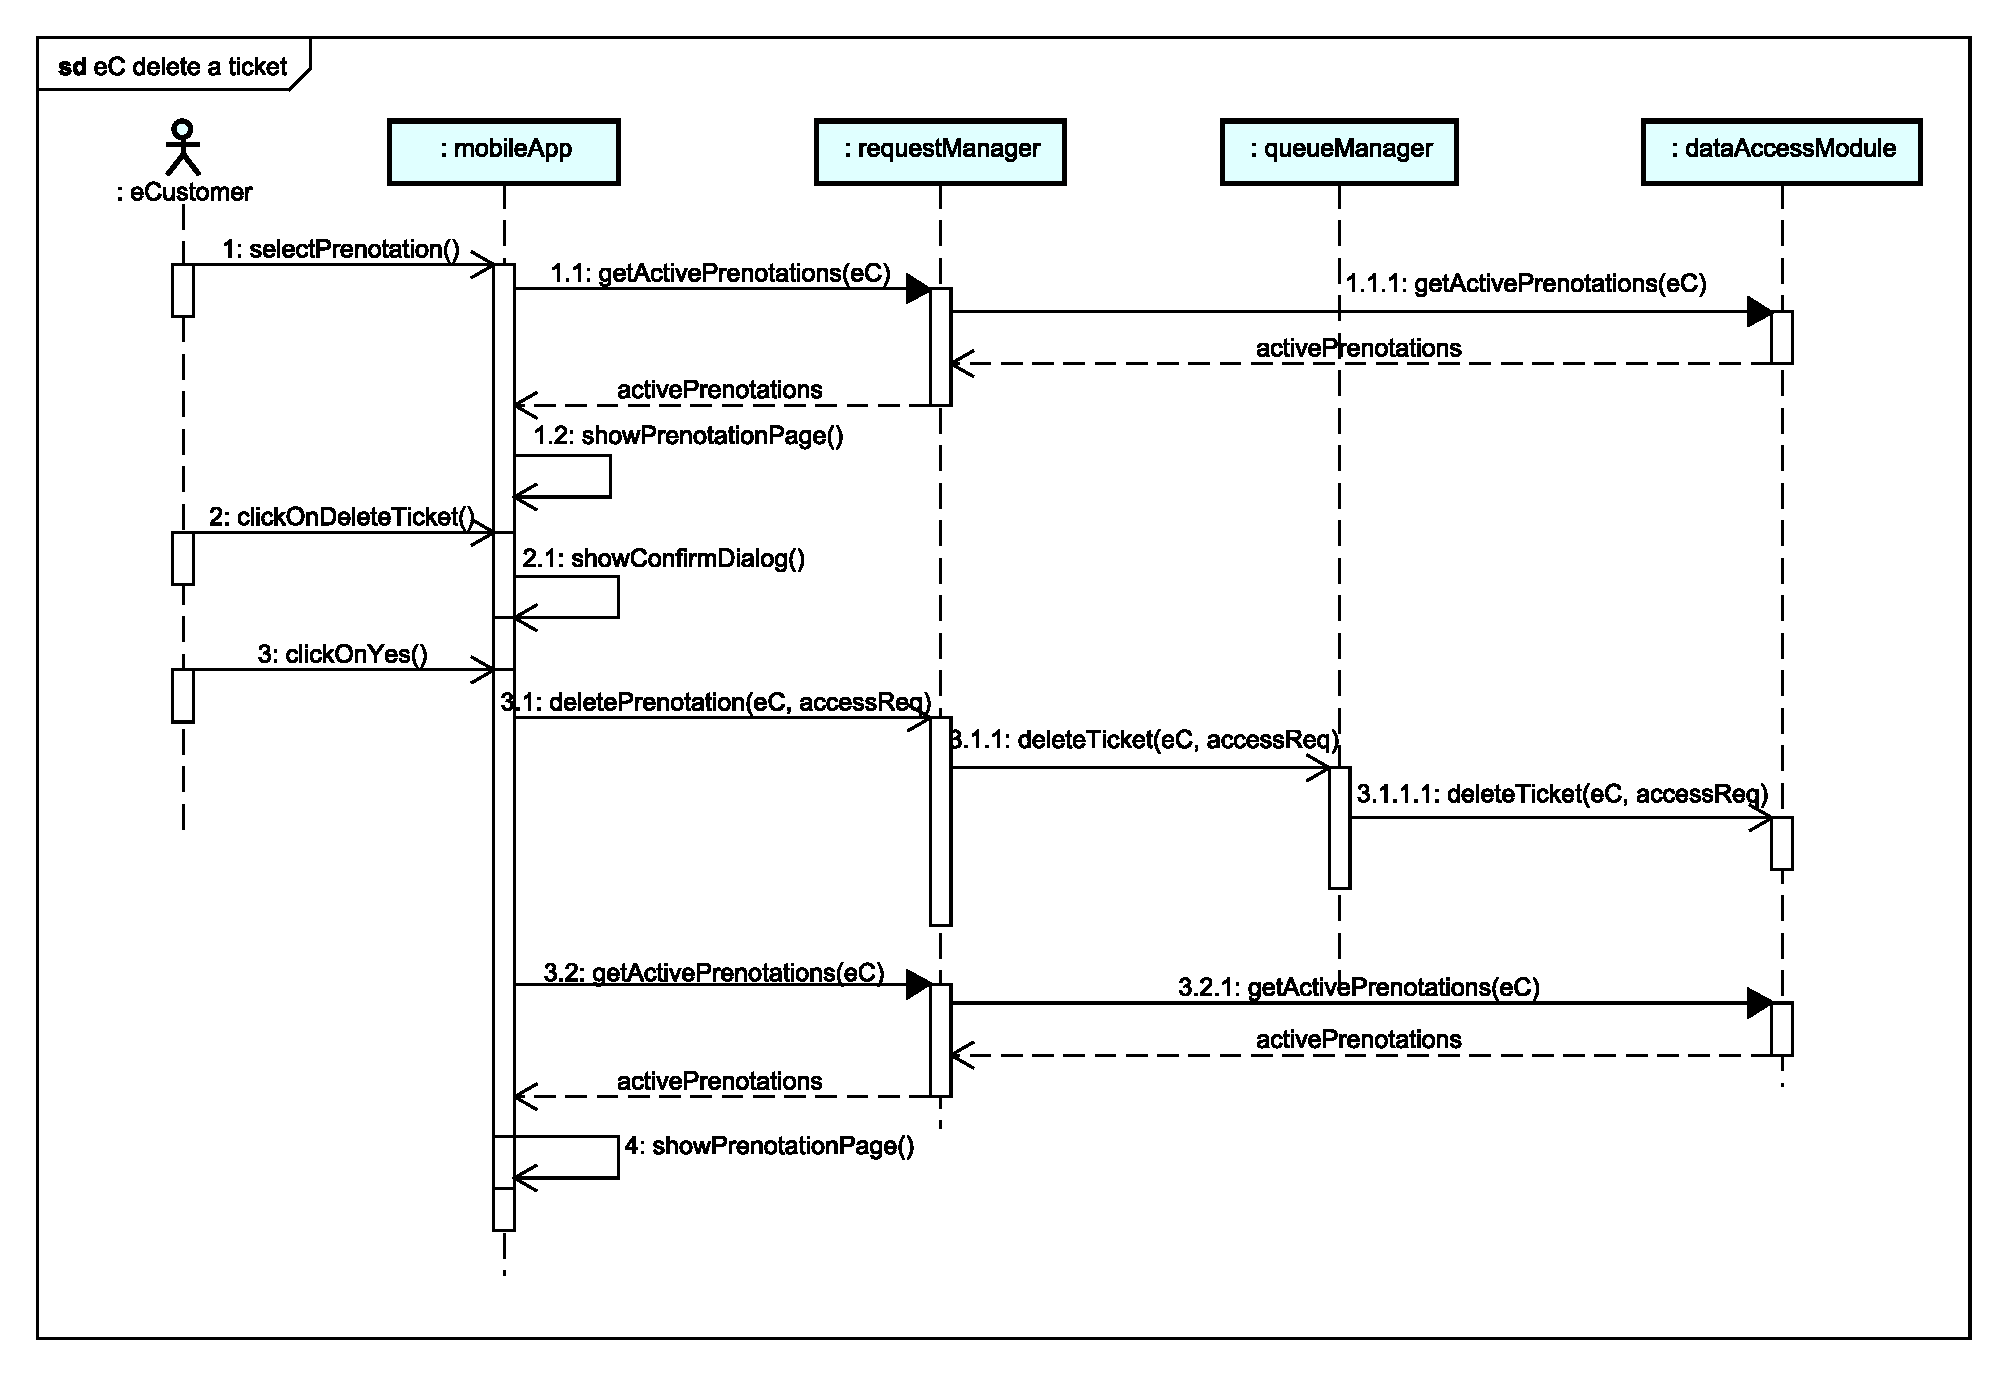
\includegraphics[width=.75\linewidth] {sequence_diagrams/eC_delete_a_ticket_seqD}
	\caption{Runtime view of an e-Customer deleting a ticket}
	\label{ecdelete} 

	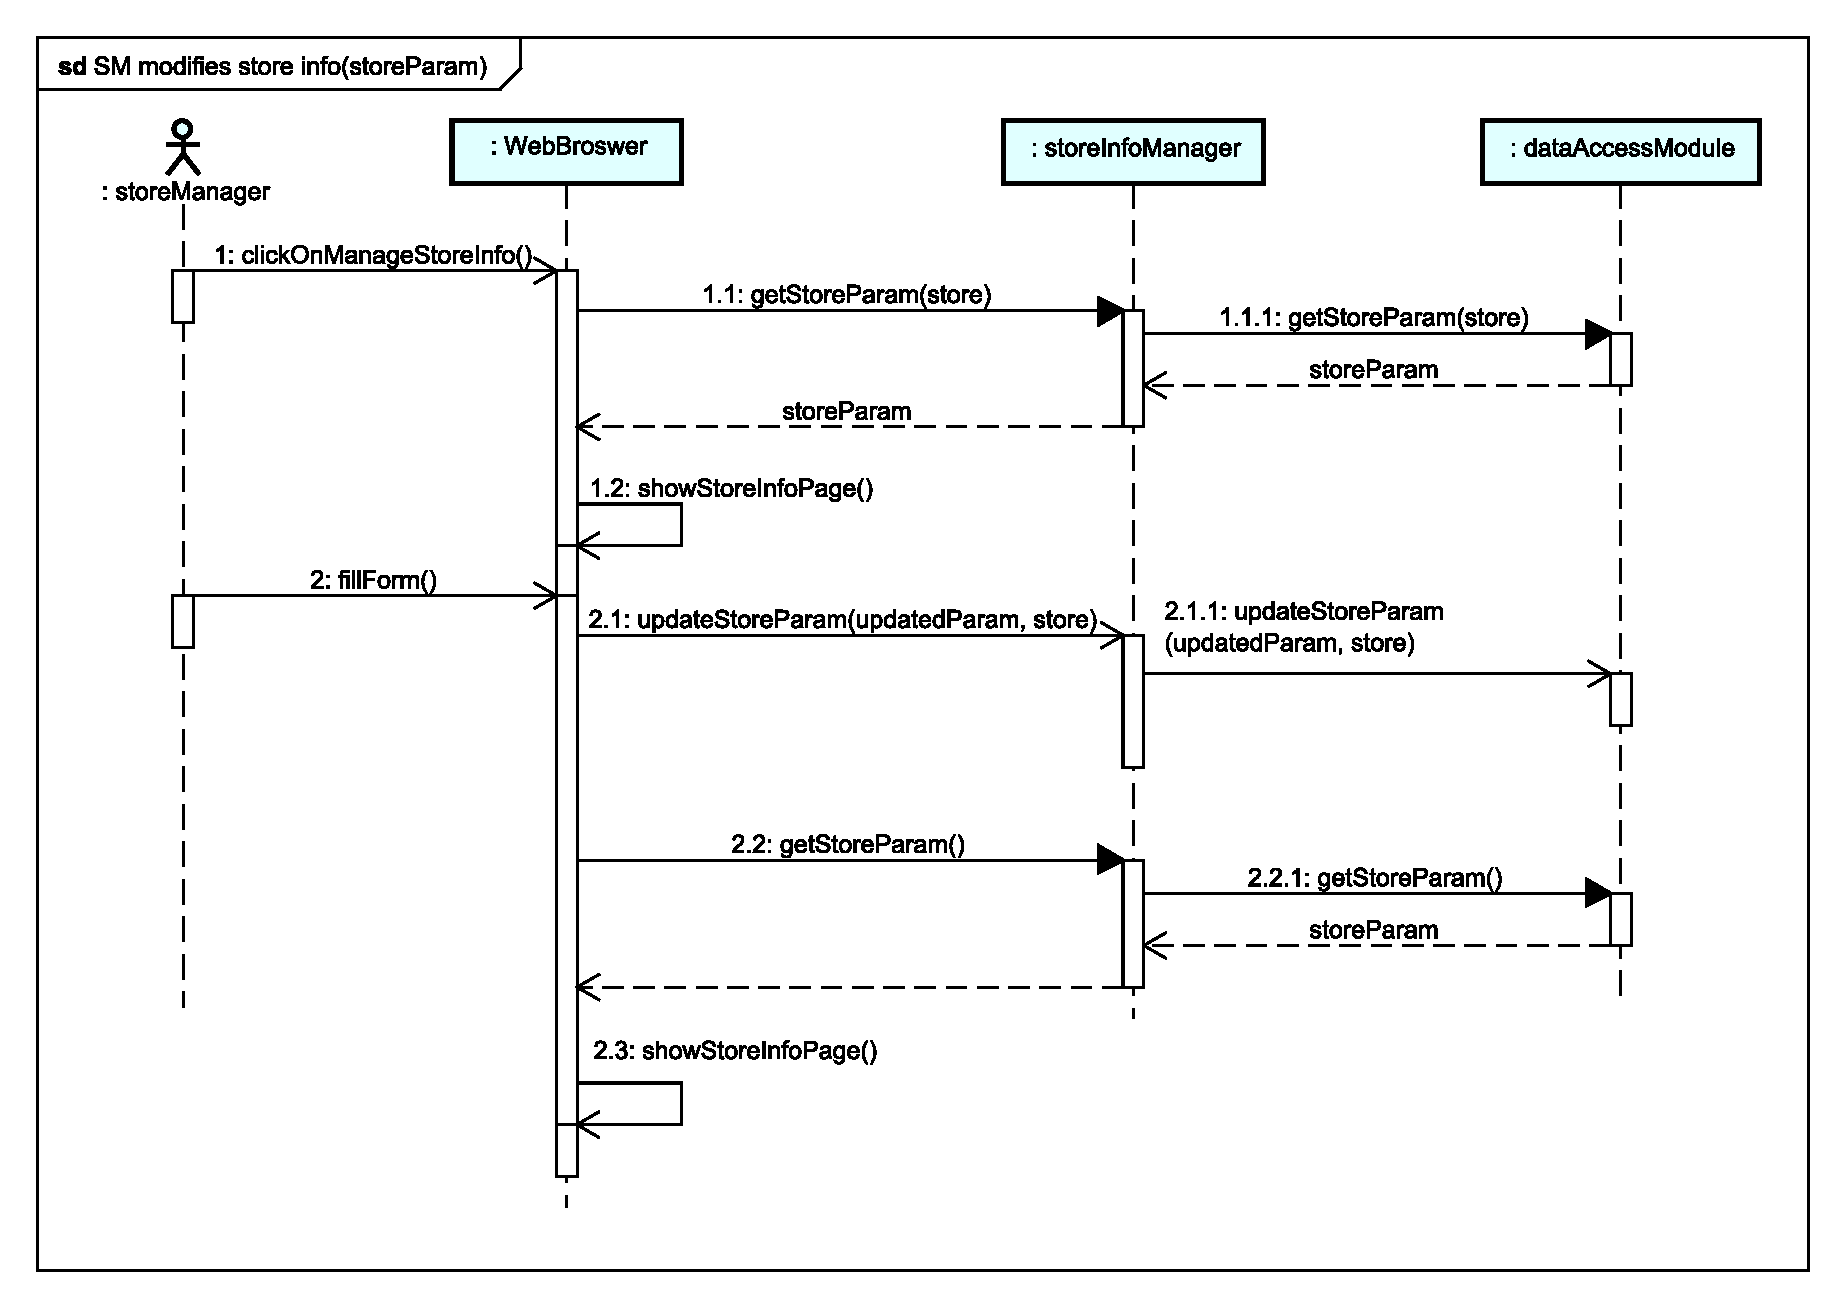
\includegraphics[width=.75\linewidth] {sequence_diagrams/SM_modifies_store_info_seqD}
	\caption{Runtime view of a Store Manager modifying their store's information}
	\label{smmodinfo} 
\end{figure}

\begin{figure}[p]	
	\centering
	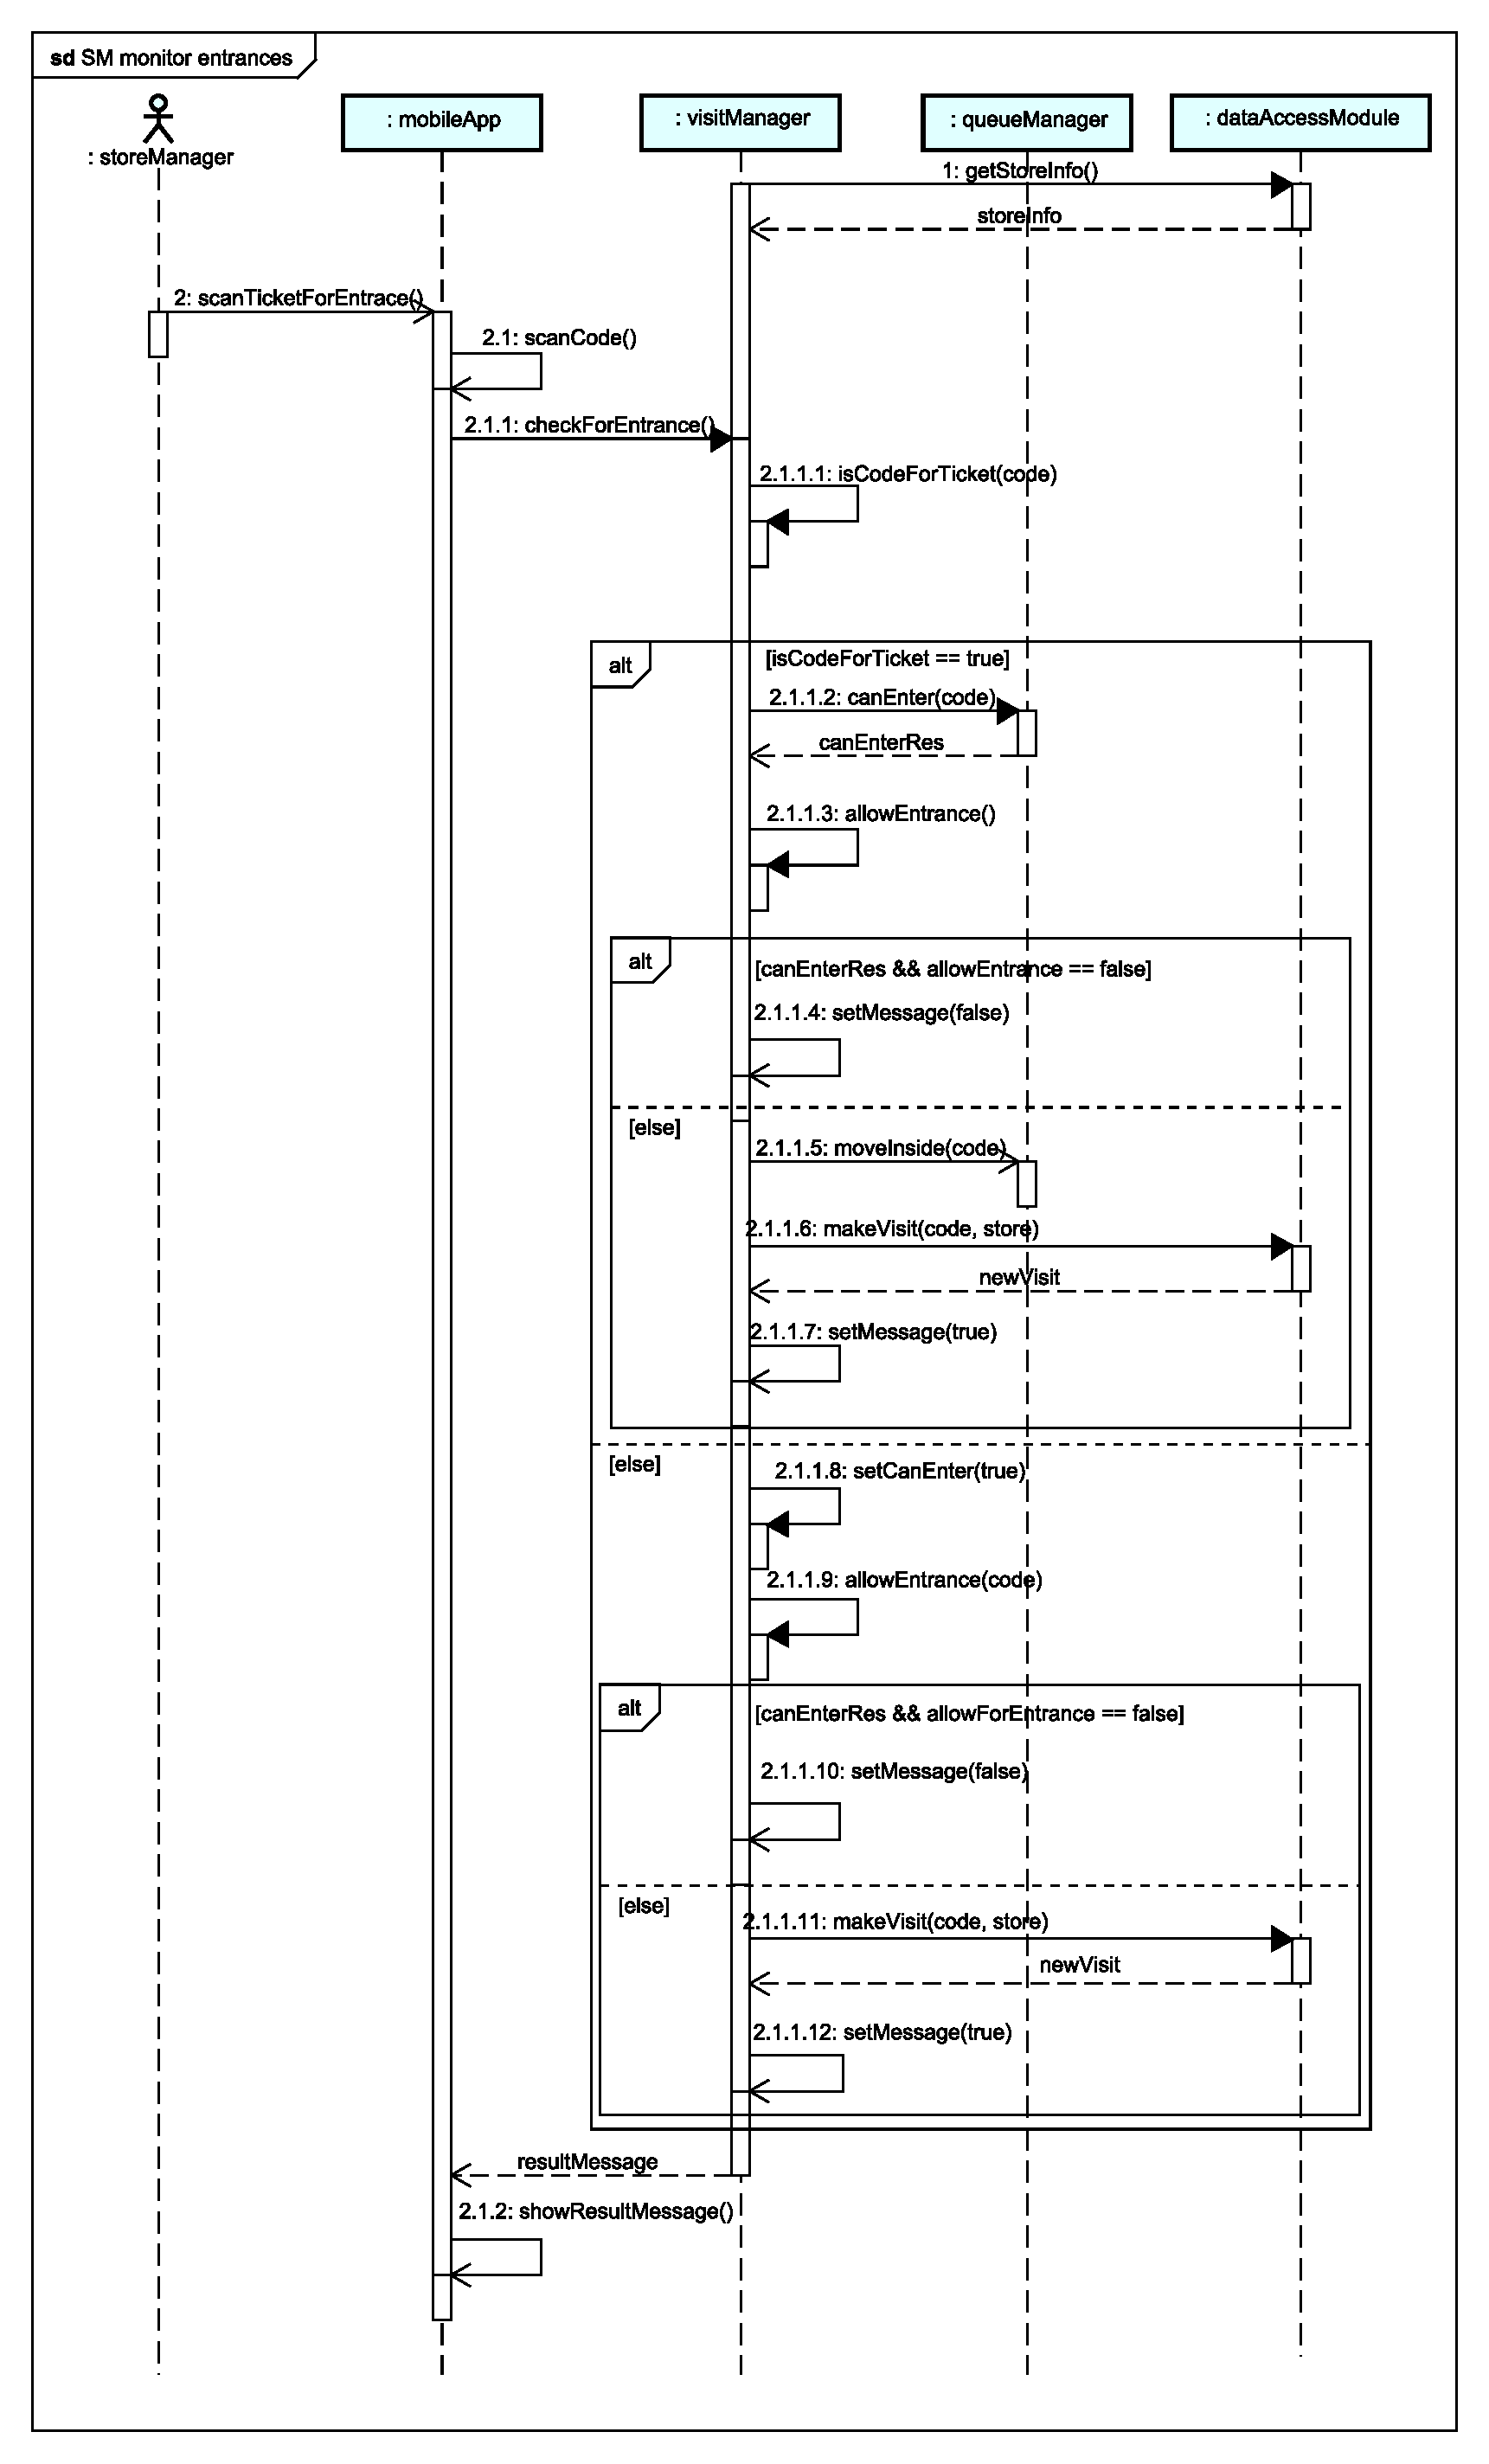
\includegraphics[height=.98\textheight] {sequence_diagrams/SM_monitor_entrances_seqD}
	\caption{Runtime view of a Store Manager monitoring accesses}
	\label{runsmmonitor} 
\end{figure}

\clearpage
% Component interfaces section, to be included in architecture.tex

\subsection{Component interfaces}
Figure \ref{intec}, Figure \ref{intsm} and Figure \ref{intstat} show the interfaces exposed by subsystems to interact with other components.

\begin{figure}[h]	
	\centering
	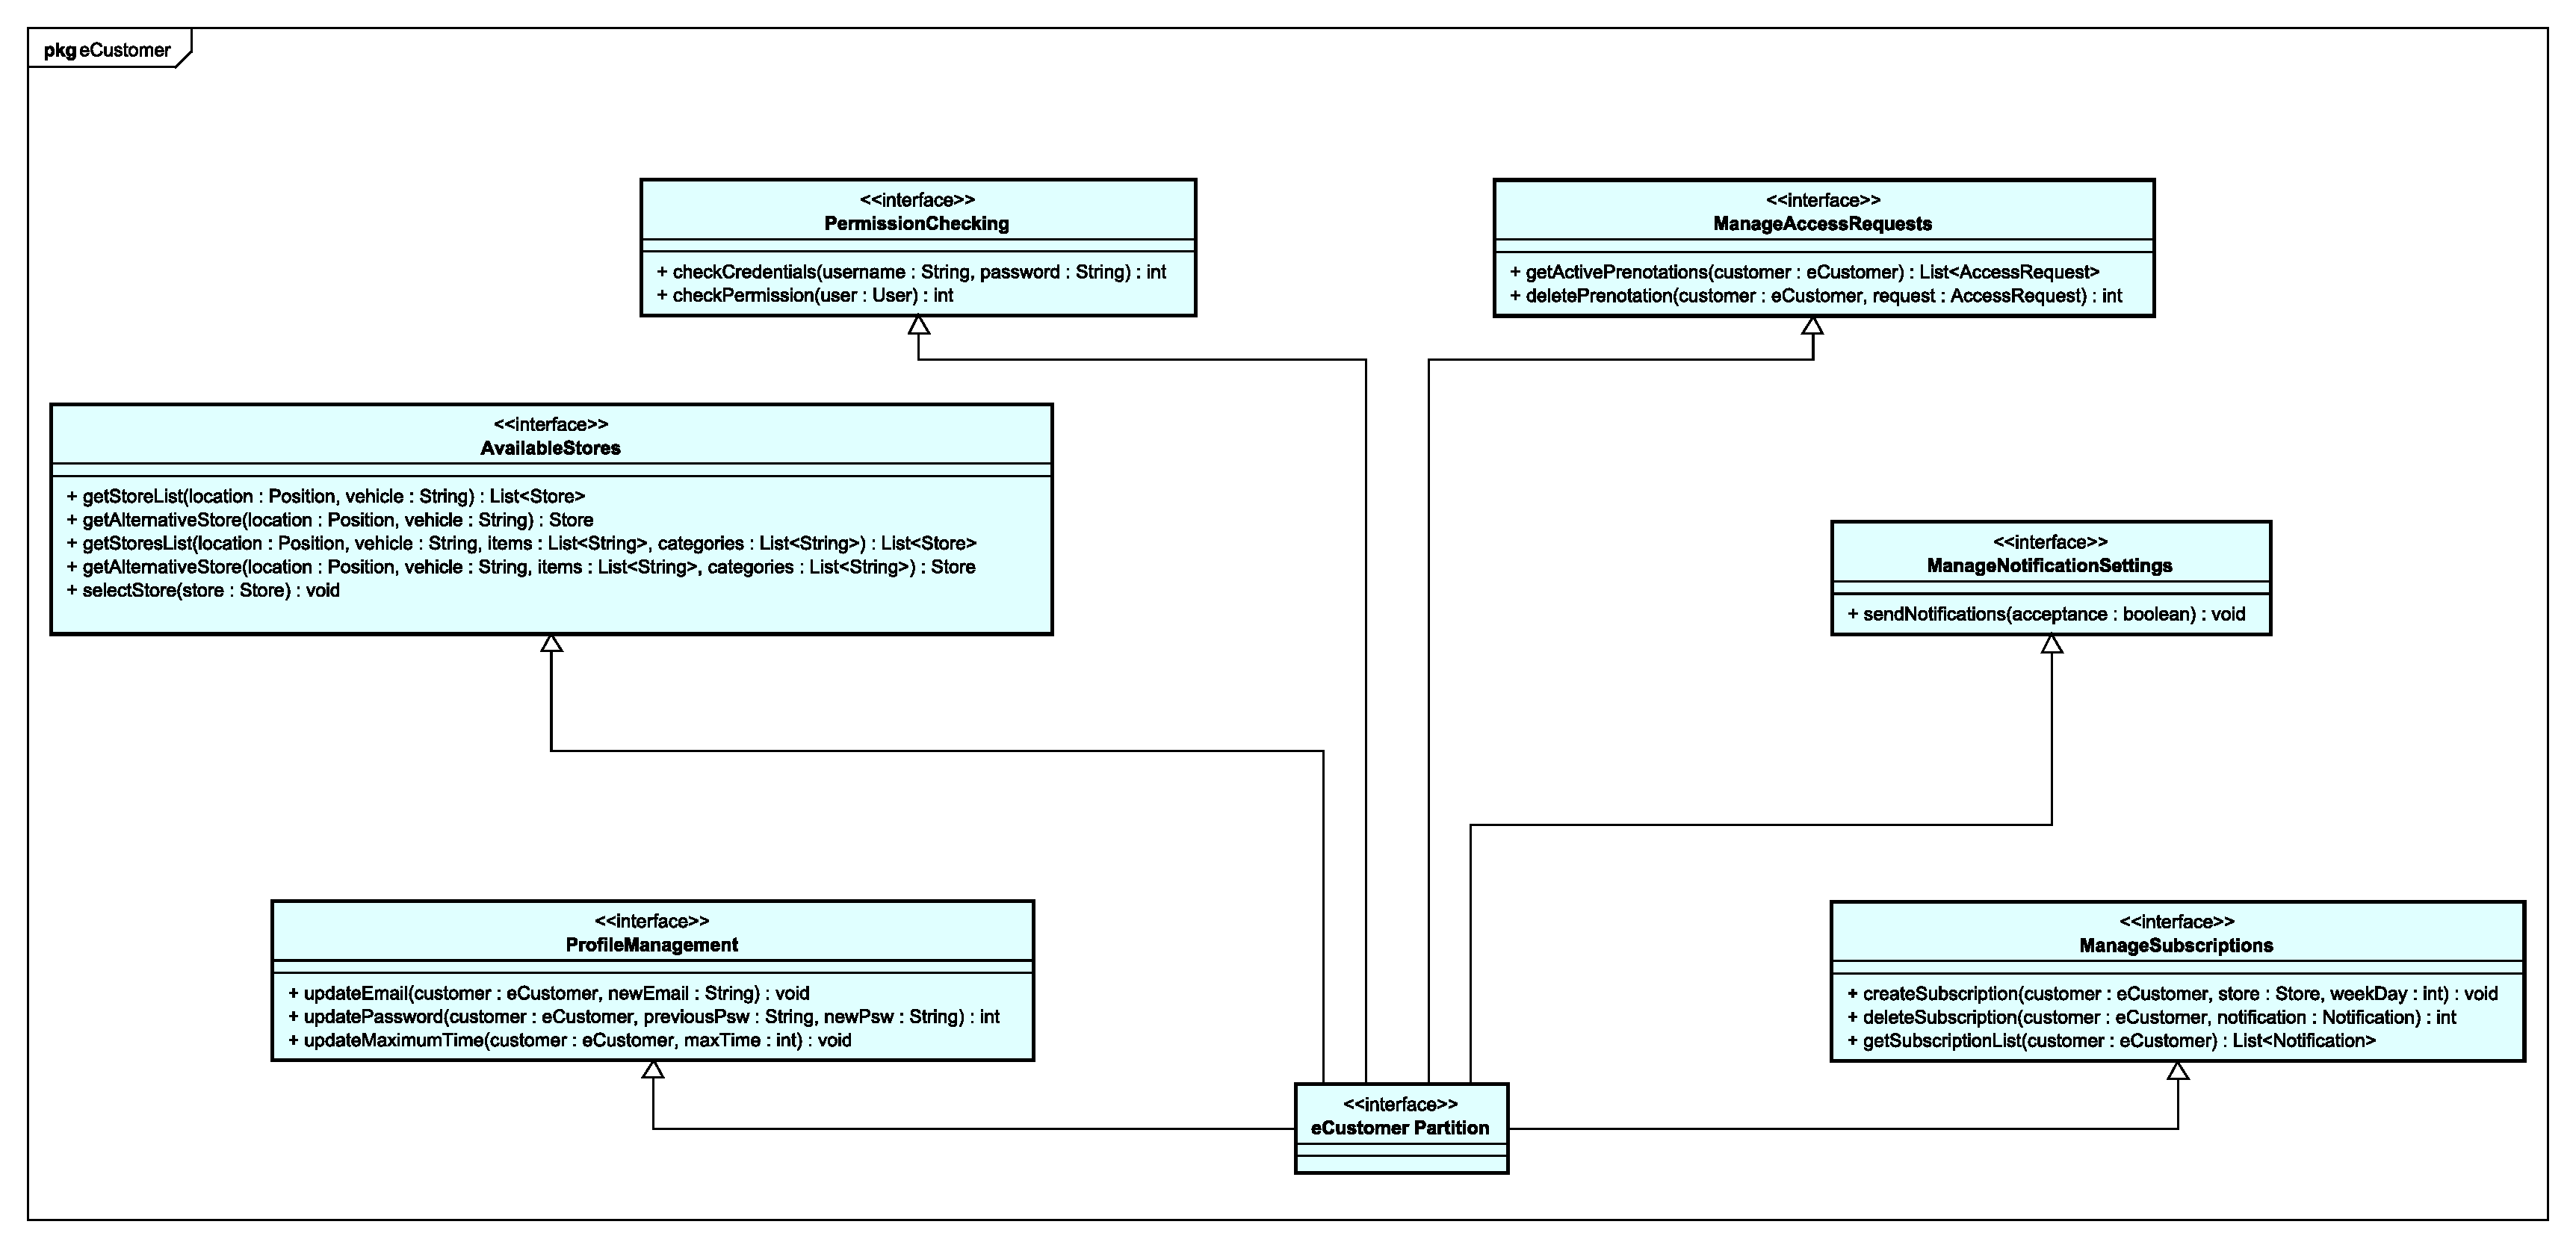
\includegraphics[width=\linewidth] {class_diagram/interface_customer}
	\caption{Component interfaces for the e-Customer subsystem}
	\label{intec}
	
	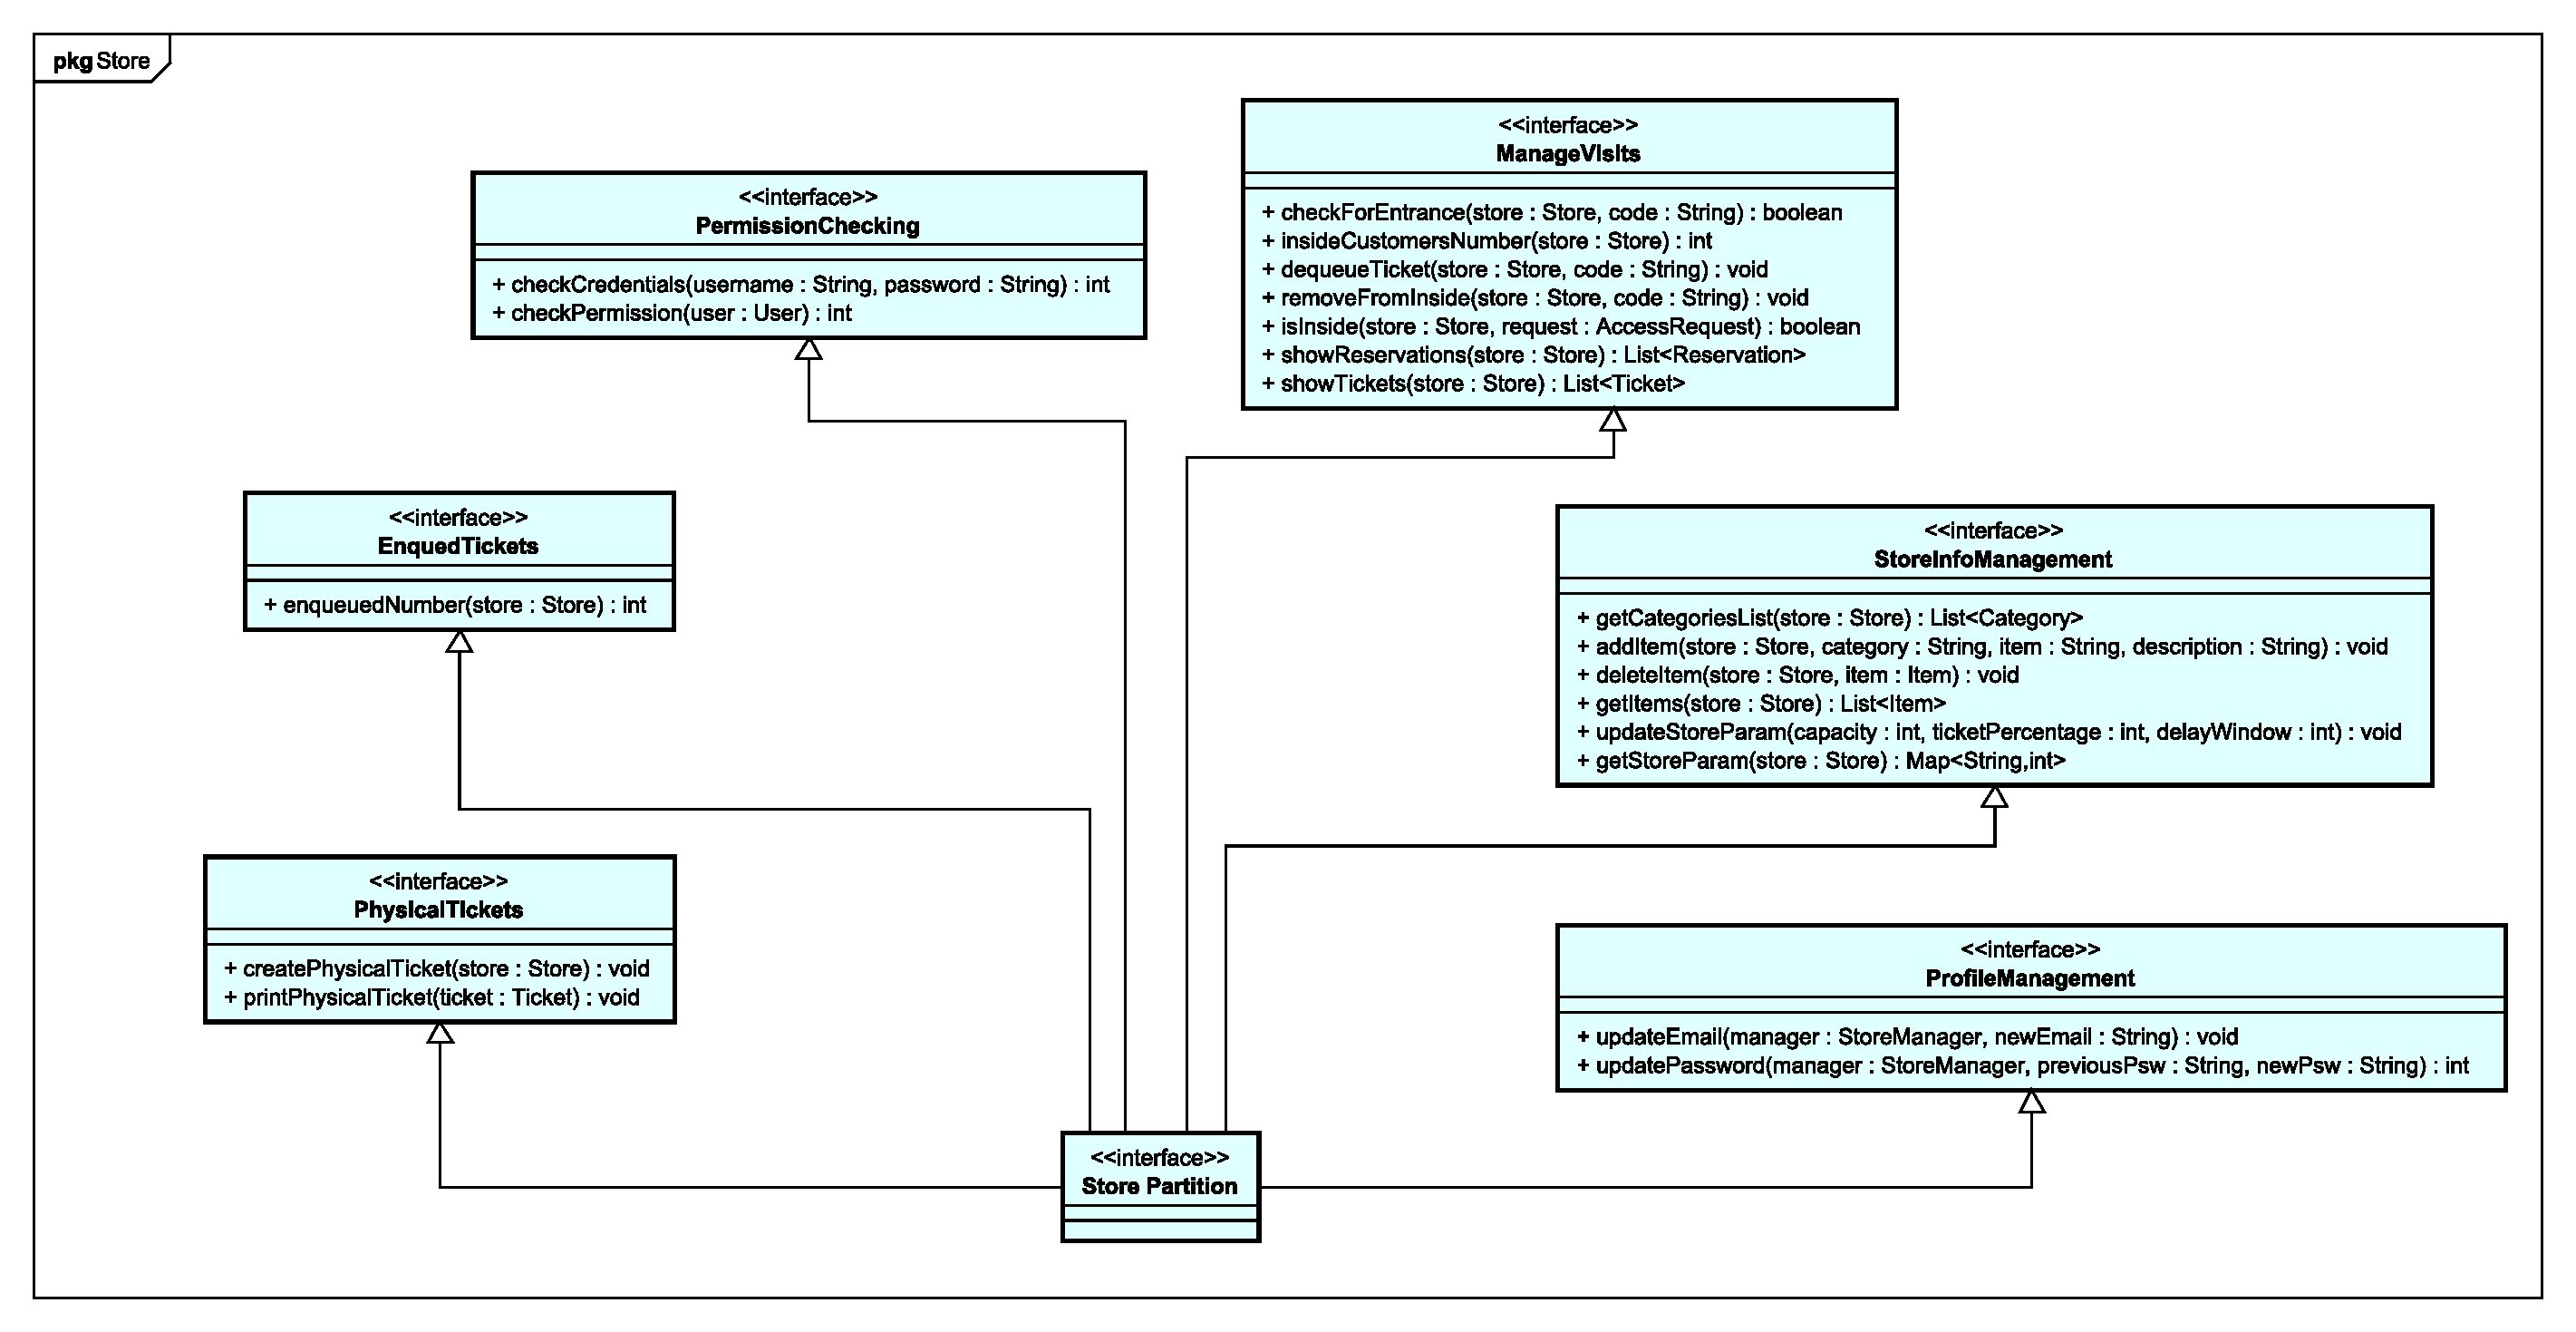
\includegraphics[width=\linewidth] {class_diagram/interface_store}
	\caption{Component interfaces for the Store Manager subsystem}
	\label{intsm}
\end{figure}

\clearpage
\begin{figure}[h]	
	\centering	
	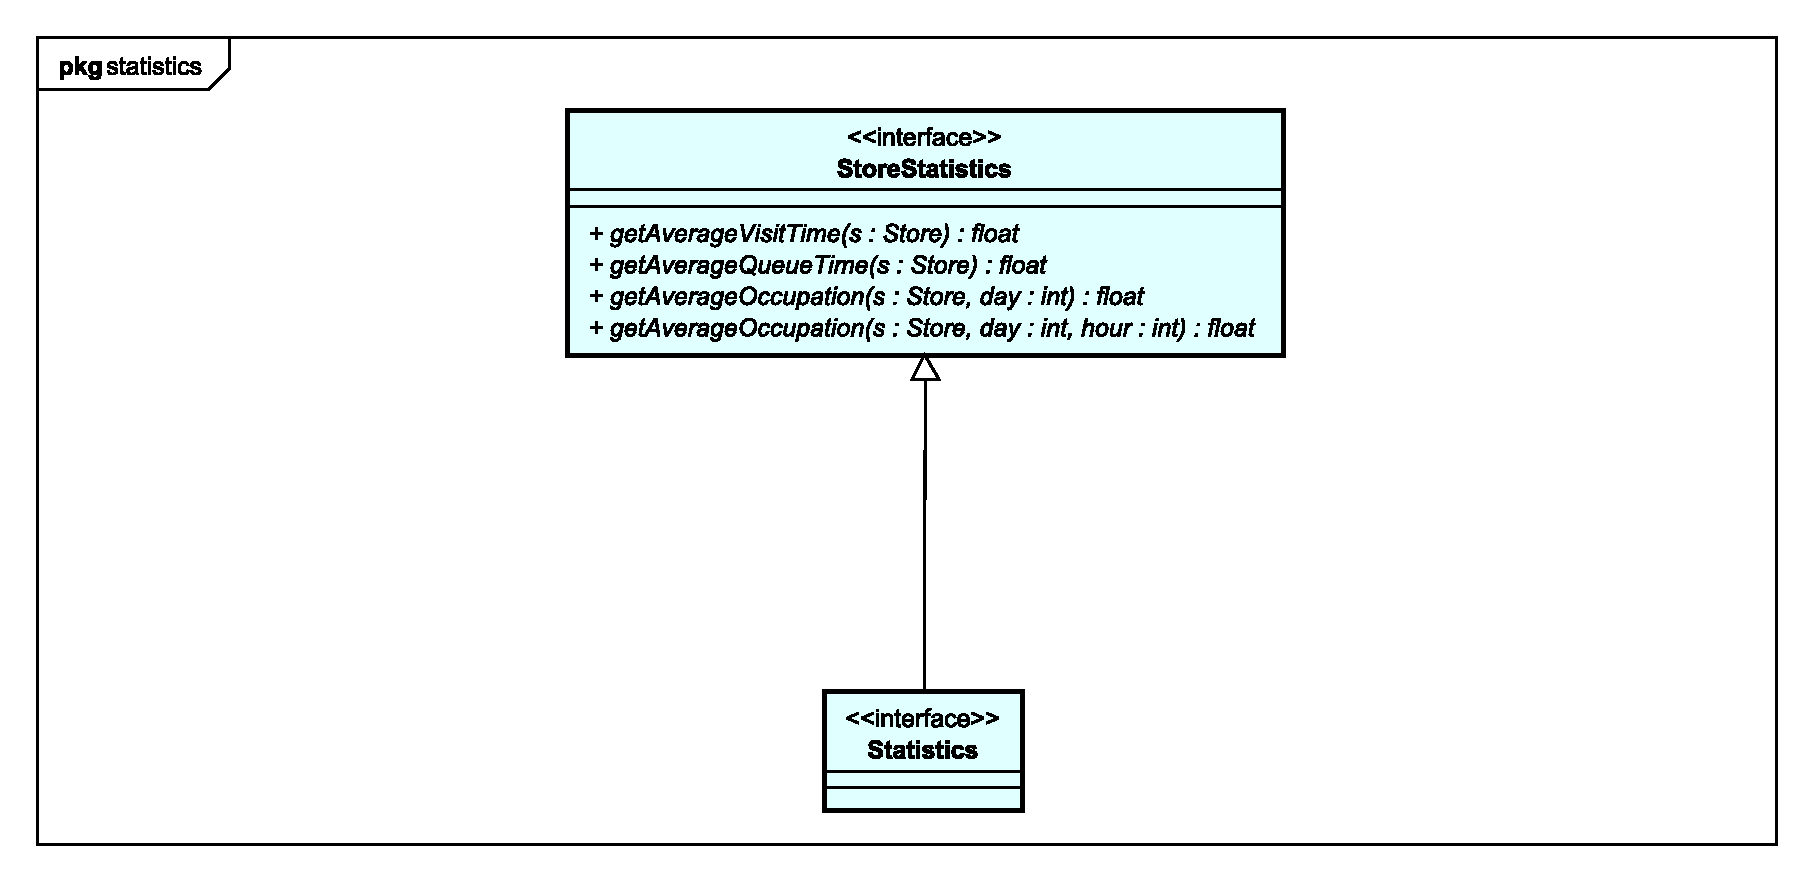
\includegraphics[width=.93\linewidth] {class_diagram/interface_statistics}
	\caption{Component interfaces for the Statistics subsystem}
	\label{intstat}
\end{figure}

\subsection{Selected architectural styles and patterns}
This section reports some directions on the use of design patterns during the implementation of the CLup system. As previously stated, the system is based on a modular design, but the following patterns are suggested:

\begin{itemize}[itemsep=-1mm, topsep=-1mm]
	\item The base architecture pattern is MVC (Model-View-Controller), as it allows to decouple the application logic from the user interaction
	\item To support MVC, the Observer Pattern\textsuperscript{\cite{observer}} should be used
	\item To have an extended interface to the database the DAO\textsuperscript{\cite{dao3}} (Data Access Object) architectural pattern is used to separate the business logic from the data tier, to moreover improve testing simplicity, to increase code readability and to make the independent from the data access technology   
	\item The application's and the online mapping system is done through an Adapter, in order to create a layer between the application and the API, and have a unified interface\textsuperscript{\cite{adapter}} for all the system's components.
	\item For what concerns the Statistic Module, a façade pattern\textsuperscript{\cite{facade}} is used to offer a unique and easy-to-use interface to its components.
	\item The frontend should use a Command pattern\textsuperscript{\cite{command}} to hide the difference among functionalities offered from the UI from a code perspective
	\item The notification module should work as a Servant to the modules using it
\end{itemize}\vspace{.5\baselineskip} 

\subsection{Other design decisions}

% Queue jumping algorithms, to be included in architecture.tex

\subsubsection{Algorithm for queue rearrangement}
In order to maximize a store occupancy, the system adopts an algorithm to let customers jump forward if a place is freed because someone dequeued; it is shown here through pseudocode. 

What is important to note is that this behaviour is based on empty places mapped 1:1 to e-Customers through notifications (physical tickets are not allowed to shift), as shown in Figure \ref{window}: every e-Customer is allowed to jump only to one place, so that their original order can be respected (if everyone accepts). An e-Customer that rejects the jump or lets the time window expire won't be asked again (in red), while, in an extreme case like the one shown (with multiple drop during one period) a customer might be asked to jump several times.

\begin{figure}[h]	
	\centering
	\includegraphics[width=.7\linewidth] {algorithms/queue}
	\caption{Visualization of the queue algorithm}
	\label{window}
\end{figure}

\paragraph{Variables}
This pseudocode assumes the existence of a queue of tickets, treated for simplicity as an array.

\paragraph{Notifier}
Every 5 minutes, a number of customers at most equal to the number of empty places is notified of an available jump, for which they won't be notified again (to avoid both multiple notifications and being notified either after a rejection or an expiration of the given time). The empty places notification order reflects the current e-Customer order.  

\begin{lstlisting}
doNotNotify = []
while(true)	
	holes = queue.getHoles()
	nextPlace = -1
	foreach(h in holes)
		nextPlace = max(nextPlace + 1, h + 1)
		while(nextplace in holes 
			or queue[nextplace] in doNotNotify)
			nextplace++
		queue[nextplace].getCustomer().notifyJumpTo(h)
		doNotNotify.add(queue[nextplace], h)
	sleep(300)
\end{lstlisting}

\paragraph{Jump}
If a customer accepts the jump, their place in queue is updated:
\begin{lstlisting}
moveTo(ticket, jumpDest)
\end{lstlisting}
% Algorithm used to generate a QR code, to be included in architecture.tex

\subsubsection{QR code generator}
This section shows how QR codes can be generated in order to ensure security and meet other design decisions of the applications. The format of the string changes based on the type of the access request, but the suggested general form consists of
\begin{center}
	\texttt{control\_character + MD5(emissionDT + storeID + accessParam)}
\end{center}
Where the \texttt{control\_character} identifies the type of request through a number and the accessParam, exclusive to the type: 
\begin{itemize}[itemsep=-1mm, topsep=-1mm]
	\item Ticket:
	\begin{itemize}[itemsep=-1mm, topsep=-1mm]
		\item \texttt{control\_character}: 0
		\item \texttt{accessParam}: nOrder
	\end{itemize}
	\item Reservation:
	\begin{itemize}[itemsep=-1mm, topsep=-1mm]
		\item \texttt{control\_character}: 1
		\item \texttt{accessParam}: entranceTime 
	\end{itemize}			
\end{itemize}\vspace{.5\baselineskip}

Through the use of MD5 all codes are guaranteed to be of length 33 characters. Figure \ref{qr} shows an example of generated QR code for a ticket with parameters:
\begin{itemize}[itemsep=-1mm, topsep=-1mm]
	\item emissionDT: 2020-12-31 10:53:31 (without spaces and special characters)
	\item storeID: 154
	\item nOrder: 51
\end{itemize}\vspace{.5\baselineskip}
That corresponds to the string
\begin{center}
	\texttt{0dd8e72b69b8e4fac5c3f3bef07e09a4a}
\end{center}

\begin{figure}[h]	
	\centering
	
\includegraphics[width=.2\linewidth] {algorithms/qr-code}
	\caption{Generated QR code}
	\label{qr}
\end{figure}

 